\section*{Appendix}
%\input{sections/proof}
%\input{sections/metrics}
%\input{sections/visualization}


\section{Motivation for VSF}
\label{app_motivate}

A limitation of standard non-latent Streaming Flow (SF) \citep{jiang2025streaming} appears when multiple
future trajectories share (almost) the same physical state before
bifurcating. The following
symmetric two-branch example isolates this issue: even at the population optimum, standard SF can exhibit a fidelity-robustness tradeoff near a bifurcation.

\begin{figure}[!b]
    \centering
    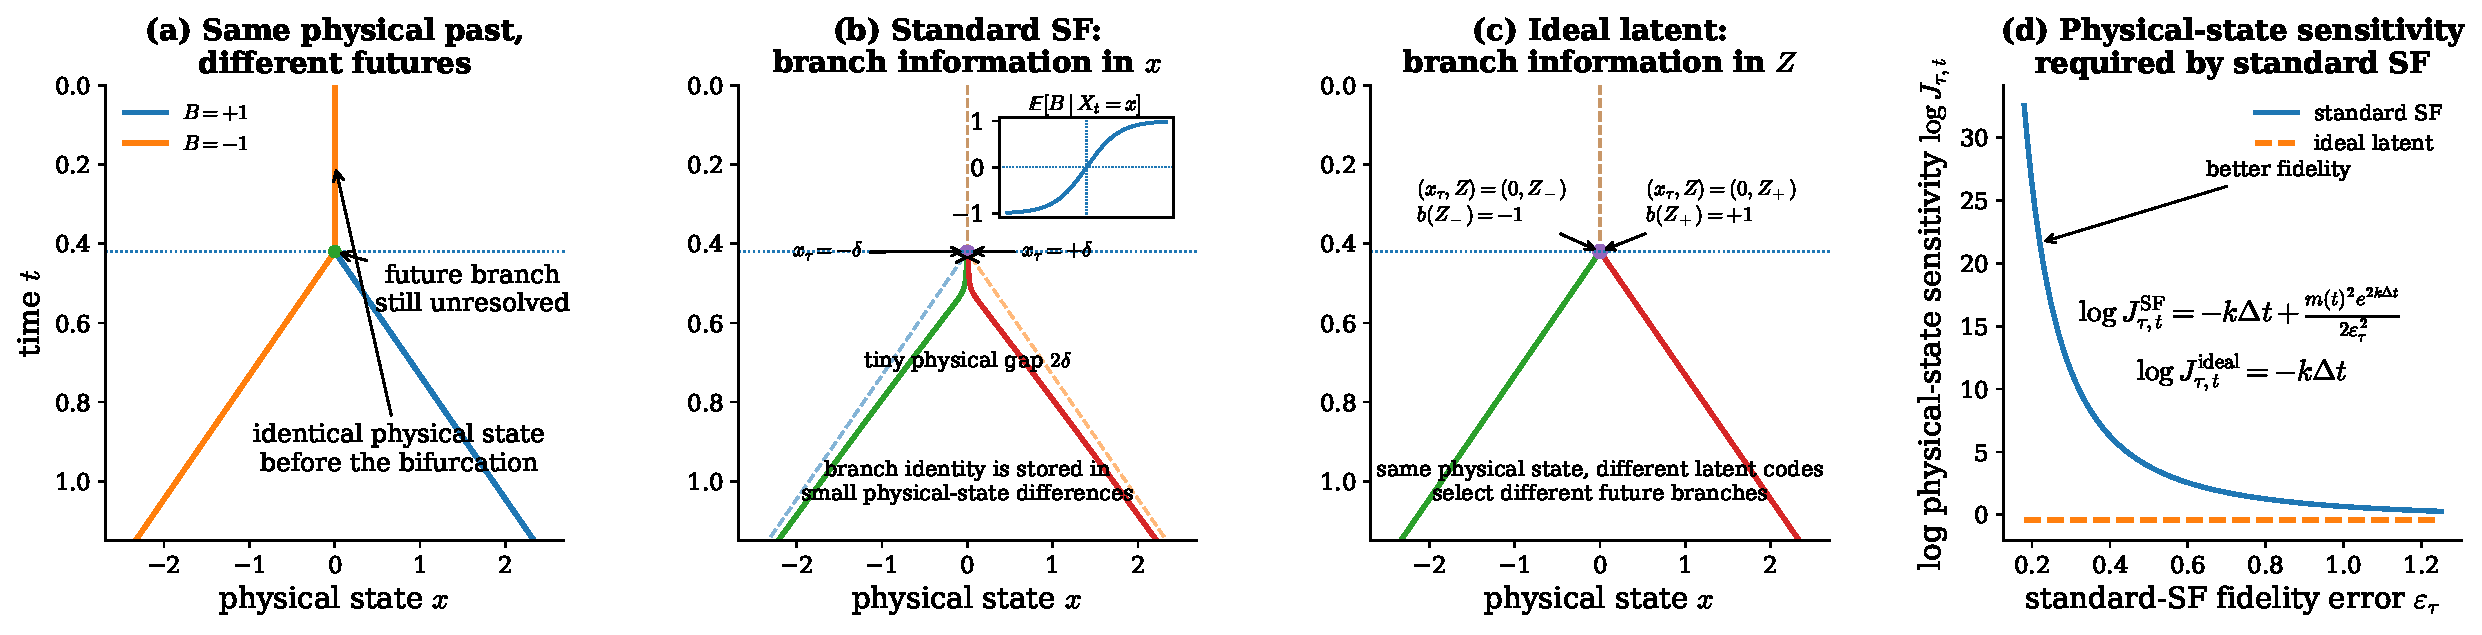
\includegraphics[width=1.005\linewidth]{figures/bif_example.pdf}
            \caption{(a) Two futures share the same physical state up to the bifurcation time $\tau$.
(b) In non-latent SF, branch identity must be encoded by small differences in the physical state $x$, making the branch signal increasingly sharp as the Gaussian tube narrows.
(c) An ideal latent realization instead carries branch identity in $Z$, allowing the same physical state $X_\tau=0$ to generate either future.
(d) Accordingly, the standard-SF physical-state sensitivity grows as
$J_{\tau,t}^{\mathrm{SF}}\sim \exp(C/\varepsilon_\tau^2)$
as the  fidelity error $\varepsilon_\tau\to0$, while the ideal latent realization retains
$J_{\tau,t}^{\mathrm{ideal}}=e^{-k(t-\tau)}$. }
    \label{fig:motivate}
\end{figure}

{\bf A bifurcation example.} Fix an observed history $H=h$. Let $B\in\{-1,+1\}$ be equally likely
conditional on $h$, and consider the two future trajectories
\begin{equation}
    \xi_B(t)=B\,m(t),
    \qquad t\in[0,T],
    \label{eq:bifurcation_paths}
\end{equation}
where $m:[0,T]\to[0,\infty)$ is absolutely continuous on $[0,T]$,
continuously differentiable on $(\tau,T]$, satisfies
$m(t)=0$ for $t\leq\tau$, and $m(t)>0$ for $t>\tau$.
Thus the two futures share the same physical trajectory up to the
bifurcation time $\tau$ and separate afterward.

Let
$k>0$ and $\sigma_0>0$, and consider the branch-conditioned fields
\begin{equation}
    g_B(x,t)
    =
    \dot\xi_B(t)-k\bigl(x-\xi_B(t)\bigr).
    \label{eq:bifurcation_sf_conditional_field}
\end{equation}
Define
$\sigma_t^2=\sigma_0^2e^{-2kt},$
$q(t)=\dot m(t)+km(t)$.

\begin{vsfproposition}[Fidelity-sensitivity tradeoff]
\label{prop_motivate} Assume that the population optimum of the SF objective is attained.  Then, we have the following results.

(i) The optimal SF marginal field is
\begin{equation}
    v_{\mathrm{SF}}^\star(x,t)
    =
    -kx
    +
    q(t)
    \tanh\!\left(
        \frac{x\,m(t)}{\sigma_t^2}
    \right).
    \label{eq:bifurcation_sf_field}
\end{equation}
At the bifurcation time,
$P_{\tau}^{\mathrm{SF}}
    =
    \mathcal N(0,\sigma_\tau^2),$
    $P_{\tau}^{\mathrm{data}}
    =
    \delta_0,$
and therefore
\begin{equation}
    \varepsilon_\tau
    :=
    W_2\!\left(
        P_{\tau}^{\mathrm{SF}},
        P_{\tau}^{\mathrm{data}}
    \right)
    =
    \sigma_\tau.
    \label{eq:bifurcation_sf_fidelity}
\end{equation}

(ii) $x(t)\equiv0$ is a trajectory of
$v_{\mathrm{SF}}^\star$. 
  If
$\Phi_{\tau,t}^{\mathrm{SF}}$ denotes its flow map, then for every
$t>\tau$,
\begin{equation}
    J_{\tau,t}^{\mathrm{SF}}
    :=
    \left.
    \frac{\partial
        \Phi_{\tau,t}^{\mathrm{SF}}(x)}
        {\partial x}
    \right|_{x=0}
    =
    \exp\!\left[
        -k(t-\tau)
        +
        \frac{
            m(t)^2e^{2k(t-\tau)}
        }{
            2\varepsilon_\tau^2
        }
    \right].
    \label{eq:bifurcation_fidelity_sensitivity}
\end{equation}
Hence, for every fixed $t>\tau$ with $m(t)>0$, and with
$k$, $m$, and $\tau$ fixed,
\begin{equation}
    \sigma_0\downarrow0
    \quad\Longleftrightarrow\quad
    \varepsilon_\tau\downarrow0
    \quad\Longrightarrow\quad
    J_{\tau,t}^{\mathrm{SF}}\to\infty.
    \label{eq:bifurcation_tradeoff_limit}
\end{equation}
\end{vsfproposition} 
Thus, in this example, standard SF faces
an explicit fidelity-sensitivity tradeoff: making the physical tube
arbitrarily close to the common target state forces the population
marginal field near the branch separator to become arbitrarily sensitive
to physical-state perturbations.

\paragraph{Proof.}
For branch $B$, plugging $\xi_B(t)=Bm(t)$ into
\eqref{eq:bifurcation_sf_conditional_field} gives
\begin{equation}
    g_B(x,t)
    =
    -kx+Bq(t),
    \qquad
    q(t)=\dot m(t)+km(t).
    \label{eq:bifurcation_sf_branch_field}
\end{equation}

We first derive the branch-conditioned  marginal field. Let
$E_t=X_t-\xi_B(t)$. From
\eqref{eq:bifurcation_sf_conditional_field},
\begin{equation}
    \dot E_t
    =
    \dot X_t-\dot\xi_B(t)
    =
    -kE_t.
\end{equation}
Hence
\begin{equation}
    E_t=e^{-kt}E_0.
\end{equation}
Since $\xi_B(0)=0$ and the standard SF construction uses
$X_0\sim\mathcal N(0,\sigma_0^2)$, we have
$E_0\sim\mathcal N(0,\sigma_0^2)$. Consequently,
\begin{equation}
    X_t\mid B
    \sim
    \mathcal N\!\left(
        Bm(t),
        \sigma_t^2
    \right),
    \qquad
    \sigma_t^2=\sigma_0^2e^{-2kt}.
    \label{eq:bifurcation_sf_branch_marginal}
\end{equation}

Under conditional flow matching, the population-optimal
marginal field is the conditional expectation of the branch-conditioned
target:
\begin{equation}
    v_{\mathrm{SF}}^\star(x,t)
    =
    \mathbb E[
        g_B(X_t,t)\mid X_t=x],
    \label{eq:bifurcation_sf_conditional_mean}
\end{equation}
where the corresponding marginal probability path is:
\begin{equation}
    P_t^{\mathrm{SF}}
    =
    \frac12\mathcal N(m(t),\sigma_t^2)
    +
    \frac12\mathcal N(-m(t),\sigma_t^2).
    \label{eq:bifurcation_sf_mixture}
\end{equation}

Using \eqref{eq:bifurcation_sf_branch_field},
\begin{equation}
    v_{\mathrm{SF}}^\star(x,t)
    =
    -kx
    +
    q(t)\,
    \mathbb E[B\mid X_t=x].
    \label{eq:bifurcation_sf_branch_mean}
\end{equation}
It remains to evaluate the posterior mean of $B$. From
\eqref{eq:bifurcation_sf_branch_marginal} and the equal branch
probabilities,
\begin{equation}
    \frac{
        \mathbb P(B=+1\mid X_t=x)
    }{
        \mathbb P(B=-1\mid X_t=x)
    }
    =
    \frac{
        \exp\!\left(
            -(x-m(t))^2/(2\sigma_t^2)
        \right)
    }{
        \exp\!\left(
            -(x+m(t))^2/(2\sigma_t^2)
        \right)
    }.
\end{equation}
Therefore
\begin{align}
    \log
    \frac{
        \mathbb P(B=+1\mid X_t=x)
    }{
        \mathbb P(B=-1\mid X_t=x)
    }
    &=
    \frac{
        (x+m(t))^2-(x-m(t))^2
    }{
        2\sigma_t^2
    }
    \notag\\
    &=
    \frac{2x\,m(t)}{\sigma_t^2}.
\end{align}
For a random variable taking values in $\{-1,+1\}$, this gives:
\begin{equation}
    \mathbb E[B\mid X_t=x]
    =
    \tanh\!\left(
        \frac{x\,m(t)}{\sigma_t^2}
    \right).
\end{equation}
Substitution into
\eqref{eq:bifurcation_sf_branch_mean} allows us to obtain
\eqref{eq:bifurcation_sf_field}.

At the bifurcation time, $m(\tau)=0$. Hence
\eqref{eq:bifurcation_sf_branch_marginal} gives
\begin{equation}
    P_{\tau}^{\mathrm{SF}}
    =
    \mathcal N(0,\sigma_\tau^2),
\end{equation}
whereas the two noiseless target branches both satisfy
$\xi_B(\tau)=0$, so
\begin{equation}
    P_{\tau}^{\mathrm{data}}=\delta_0.
\end{equation}
The only coupling between a distribution and a Dirac mass sends every
sample to the location of the Dirac mass. Therefore
\begin{align}
    W_2^2\!\left(
        P_{\tau}^{\mathrm{SF}},
        \delta_0
    \right)
    &=
    \mathbb E|X_\tau|^2
    = \sigma_\tau^2.
\end{align}
Thus
$W_2\!\left(
        P_{\tau}^{\mathrm{SF}},
        P_{\tau}^{\mathrm{data}}
    \right)  =
    \sigma_\tau,$
which is precisely
\eqref{eq:bifurcation_sf_fidelity}.

We next compute the sensitivity of the population SF near
the branch separator. By symmetry,
$v_{\mathrm{SF}}^\star(0,t)=0,$
so $x(t)\equiv0$ is a trajectory. Differentiating
\eqref{eq:bifurcation_sf_field} with respect to $x$ gives
\begin{equation}
    \partial_xv_{\mathrm{SF}}^\star(x,t)
    =
    -k
    +
    \frac{
        m(t)q(t)
    }{
        \sigma_t^2
    }
    \operatorname{sech}^2\!\left(
        \frac{x\,m(t)}{\sigma_t^2}
    \right).
\end{equation}
Along the central trajectory,
\begin{equation}
    \partial_xv_{\mathrm{SF}}^\star(0,t)
    =
    -k
    +
    \frac{
        m(t)[\dot m(t)+km(t)]
    }{
        \sigma_t^2
    }.
    \label{eq:bifurcation_sf_central_jacobian}
\end{equation}

Let
\begin{equation}
    J_{\tau,t}^{\mathrm{SF}}
    =
    \left.
    \frac{\partial
        \Phi_{\tau,t}^{\mathrm{SF}}(x)}
        {\partial x}
    \right|_{x=0}.
\end{equation}
The variational equation for the one-dimensional ODE flow gives
\begin{equation}
    \frac{d}{dt}J_{\tau,t}^{\mathrm{SF}}
    =
    \partial_xv_{\mathrm{SF}}^\star(0,t)
    J_{\tau,t}^{\mathrm{SF}},
    \qquad
    J_{\tau,\tau}^{\mathrm{SF}}=1.
\end{equation}
Therefore
\begin{equation}
    J_{\tau,t}^{\mathrm{SF}}
    =
    \exp\!\left(
        \int_\tau^t
        \partial_xv_{\mathrm{SF}}^\star(0,s)\,ds
    \right).
    \label{eq:bifurcation_sf_variational_solution}
\end{equation}

Since $\sigma_s^2=\sigma_0^2e^{-2ks}$,
\begin{equation}
    \frac{d}{ds}
    \left(
        \frac{m(s)^2}{2\sigma_s^2}
    \right)
    =
    \frac{
        m(s)[\dot m(s)+km(s)]
    }{
        \sigma_s^2
    }.
\end{equation}
Using $m(\tau)=0$ in
\eqref{eq:bifurcation_sf_central_jacobian}, we obtain
\begin{align}
    \int_\tau^t
    \partial_xv_{\mathrm{SF}}^\star(0,s)\,ds
    &=
    -k(t-\tau)
    +
    \int_\tau^t
    \frac{
        m(s)[\dot m(s)+km(s)]
    }{
        \sigma_s^2
    }
    ds
    \notag\\
    &=
    -k(t-\tau)
    +
    \frac{m(t)^2}{2\sigma_t^2}.
\end{align}

From
$\sigma_t^2=\sigma_\tau^2e^{-2k(t-\tau)}$ and
$\varepsilon_\tau=\sigma_\tau$, we further obtain
\begin{equation}
    \frac{m(t)^2}{2\sigma_t^2}
    =
    \frac{
        m(t)^2e^{2k(t-\tau)}
    }{
        2\varepsilon_\tau^2
    }.
\end{equation}
Using these and
\eqref{eq:bifurcation_sf_variational_solution}, we  obtain
\eqref{eq:bifurcation_fidelity_sensitivity}. 

Finally, for every fixed
$t>\tau$ with $m(t)>0$, the second term in the exponent diverges as
$\varepsilon_\tau\to0$, which proves
\eqref{eq:bifurcation_tradeoff_limit}.

\begin{vsfcorollary}
\label{cor:sf_fidelity_robustness_lower_bound}
Under the assumptions of
Proposition~\ref{prop_motivate}, suppose that for
some fixed $t>\tau$ the SF sensitivity is required to
satisfy
$J_{\tau,t}^{\mathrm{SF}}\leq J_{\max}$ for some threshold $J_{\max}$. Then,
whenever this constraint is feasible, it is necessary that
$J_{\max}>e^{-k(t-\tau)}$, and
\begin{equation}
    \varepsilon_\tau
    \geq
    \frac{
        m(t)e^{k(t-\tau)}
    }{
        \sqrt{
            2\left[
                \log J_{\max}+k(t-\tau)
            \right]
        }
    }.
    \label{eq:sf_fidelity_lower_bound}
\end{equation}
\end{vsfcorollary}
Thus, within this model,  keeping the
physical-state sensitivity bounded by a threshold imposes a strictly positive lower bound on
the fidelity error.


\begin{tcolorbox}[
  colback=parchment,
  colframe=sandborder,
  boxrule=0.1pt,
  left=8pt,
  right=8pt,
  top=0.3pt,
  bottom=0.3pt
]
\centering
Proposition \ref{prop_motivate} reveals a limitation in  SF:  the physical state must simultaneously track the shared trajectory and encode  future branch information, so near a bifurcation improved physical fidelity necessarily causes branch selection to be more sensitive to state perturbations.
\end{tcolorbox}

%Along the common stem, both true future branches satisfy $X_t=0$, whereas the SF state retains variance $\sigma_t^2$. Shrinking this physical tube improves fidelity, but the marginal field must then infer opposite branch directions from increasingly nearby physical states. 
%The factor $\tanh\!\left(\frac{x\,m(t)}\sigma_t^2}\right)$ makes this explicit: as $\sigma_t$ decreases, the branch-separating transition around $x=0$ becomes increasingly sharp. 
\Eqref{eq:bifurcation_fidelity_sensitivity} quantifies the resulting
fidelity--sensitivity tradeoff.

\paragraph{Why introducing a latent model?} While latent variable models are more expressive and can improve performance in general,
the preceding example gives a clear motivation to separate the stochastic branch
information from the physical state, motivating the use of latent SF models.
In the following, we show that there exists such a latent model, without making
a claim about the learned model itself. 
Let $Z\sim\mathcal N(0,1)$ be sampled once for the
trajectory, define
\begin{equation}
b(Z)
=
\begin{cases}
+1, & Z\geq0,\\
-1, & Z<0,
\end{cases}
\label{eq:bifurcation_ideal_branch_code}
\end{equation}
and use the latent-conditioned physical-time field
\begin{equation}
v_{\mathrm{ideal}}(x,t,Z)
=
-kx+b(Z)q(t)
=
b(Z)\dot m(t)
-
k\bigl(x-b(Z)m(t)\bigr),
\label{eq:bifurcation_ideal_field}
\end{equation}
where $q(t)=\dot m(t)+km(t)$ as above.
Thus, conditional on the latent branch code $b(Z)$,
$v_{\mathrm{ideal}}$ has exactly the same form as the branch-conditioned
SF field in \eqref{eq:bifurcation_sf_branch_field}; the difference is that
the branch information is now supplied by the latent variable rather than
having to be inferred from the physical state.

Starting from the  observed state $X_0=0$, this field gives
\begin{equation}
X_t=b(Z)m(t),
\label{eq:bifurcation_ideal_path}
\end{equation}
and hence realizes the target conditional path law
\begin{equation}
\operatorname{Law}(X_\cdot\mid H=h)
=
\frac12\delta_{\xi_+}
+
\frac12\delta_{\xi_-}.
\label{eq:bifurcation_ideal_path_law}
\end{equation}
In particular,
$W_2\left(
P_{\tau}^{\mathrm{ideal}},
P_{\tau}^{\mathrm{data}}
\right)
=0.$
Furthermore,
\begin{equation}
\partial_xv_{\mathrm{ideal}}(x,t,Z)=-k,
\end{equation}
so, for fixed $Z$,
\begin{equation}
\frac{\partial
\Phi_{\tau,t}^{\mathrm{ideal}}(x,Z)}
{\partial x}
=
e^{-k(t-\tau)}.
\label{eq:bifurcation_ideal_sensitivity}
\end{equation}

Indeed, define
$E_t=X_t-b(Z)m(t).$
Using \eqref{eq:bifurcation_ideal_field},
\begin{align}
\dot E_t
&=
\dot X_t-b(Z)\dot m(t)
=
-k\bigl(X_t-b(Z)m(t)\bigr)
=
-kE_t.
\end{align}
Since $X_0=0$ and $m(0)=0$, we have $E_0=0$, and therefore
$E_t=0$ for every $t$, which proves
\eqref{eq:bifurcation_ideal_path}. Since
$\mathbb P(b(Z)=+1)=\mathbb P(b(Z)=-1)=1/2$, this proves
\eqref{eq:bifurcation_ideal_path_law}; since $m(\tau)=0$, we have $W_2\left(
P_{\tau}^{\mathrm{ideal}},
P_{\tau}^{\mathrm{data}}
\right)
=0$.

More generally, for fixed $Z$, solving
\eqref{eq:bifurcation_ideal_field} from time $\tau$ with
$X_\tau=x$ gives
\begin{equation}
\Phi_{\tau,t}^{\mathrm{ideal}}(x,Z)
=
e^{-k(t-\tau)}x+b(Z)m(t),
\end{equation}
where we used $m(\tau)=0$. Differentiating with respect to $x$
gives \eqref{eq:bifurcation_ideal_sensitivity}.
This construction shows what becomes possible once branch information
need not be stored in the physical coordinate: the physical state can remain
on the common stem, while the latent variable distinguishes the future
trajectories.

\paragraph{Connection to rollout robustness.}
The sensitivity calculation also gives a direct local mechanism to understand rollout
error amplification. If a small physical-state perturbation $\delta$ is
introduced at the bifurcation, then standard SF satisfies
\begin{equation}
\Phi_{\tau,t}^{\mathrm{SF}}(\delta)
-
\Phi_{\tau,t}^{\mathrm{SF}}(0)
=
J_{\tau,t}^{\mathrm{SF}}\delta
+
o(\delta),
\label{eq:bifurcation_sf_perturbation}
\end{equation}
whereas the ideal latent construction satisfies, for fixed $Z$,
\begin{equation}
\Phi_{\tau,t}^{\mathrm{ideal}}(x+\delta,Z)
-
\Phi_{\tau,t}^{\mathrm{ideal}}(x,Z)
=
e^{-k(t-\tau)}\delta.
\label{eq:bifurcation_ideal_perturbation}
\end{equation}
Thus, in this example the same mechanism behind the 
fidelity-sensitivity tradeoff also provides a mechanism by which standard
non-latent SF can amplify physical-state rollout errors near a branch
separator. By contrast, once the branch information is encoded by the
latent variable in the idealized construction, physical-state perturbations
are governed only by the original stabilizing dynamics and are contracted
at rate $e^{-k(t-\tau)}$.

\paragraph{This motivates VSF.}
The proposition and discussions above identify a bottleneck of
standard non-latent SF, and the idealized latent construction shows
how that bottleneck can in principle be removed by carrying future-specific
information outside the physical state.
This observation motivates VSF. Rather than requiring the physical state alone
to carry all residual uncertainty needed for later bifurcation, VSF conditions
the physical-time velocity field on an additional latent variable sampled once
per forecast. 
\begin{tcolorbox}[
  colback=parchment,
  colframe=sandborder,
  boxrule=0.1pt,
  left=8pt,
  right=8pt,
  top=0.3pt,
  bottom=0.3pt
]
\centering
The variational  framework of VSF provides a principled way to associate
observed future dynamics with {\it learned latent codes} during training, while the learned prior
provides the corresponding randomness at inference. 
\end{tcolorbox}
The goal is therefore to
learn a distribution of coherent physical-time dynamics in which distinct
future continuations can be represented without requiring increasingly
sensitive separation in the physical state itself.




\clearpage
\section{A variational objective for clean streaming trajectories}
\label{sec:clean_velocity_elbo}


\begin{vsfproposition}[Conditional-velocity evidence lower bound]
\label{prop:velocity_elbo}
Fix a training tuple $(\vu_s,\vx_s,s,\vh)$ constructed from the physical-time
path in Eqs.~\ref{eq:physical_time_interpolation}--
\ref{eq:physical_time_velocity}.  Let $p(\vz)$ be the latent prior, 
$p_{\vtheta}(\vu_s\mid\vx_s,s,\vh,\vz)$ be a conditional velocity
likelihood, and $q_{\vphi}(\vz\mid\vu_s,\vx_s,s,\vh)$ be a
variational posterior.  Define the conditional velocity evidence by
\begin{equation}
  p_{\vtheta}(\vu_s\mid\vx_s,s,\vh)
  :=
  \int
  p_{\vtheta}(\vu_s\mid\vx_s,s,\vh,\vz)
  p(\vz)\,d\vz.
  \label{eq:conditional_velocity_evidence}
\end{equation}
Assume that the displayed quantities are finite, that the evidence is
positive, and that the variational posterior is absolutely continuous with
respect to the exact model posterior.
Then
\begin{align}
  \log p_{\vtheta}(\vu_s\mid\vx_s,s,\vh)
  &\geq
  \mathcal E_{\vtheta,\vphi}(\vu_s,\vx_s,s,\vh)
  \notag\\
  &:={}
  \E_{q_{\vphi}}
  \!\left[
    \log p_{\vtheta}(\vu_s\mid\vx_s,s,\vh,\vz)
  \right]
  \notag
  -
  \KL\!\left(
    q_{\vphi}(\vz\mid\vu_s,\vx_s,s,\vh)
    \,\Vert\,
    p(\vz)
  \right).
  \label{eq:pointwise_velocity_elbo}
\end{align}
\end{vsfproposition}

\paragraph{Proof.}
Inserting the variational posterior into the conditional evidence gives
\begin{align*}
  \log p_{\vtheta}(\vu_s\mid\vx_s,s,\vh)
  &={}
  \log\int
  q_{\vphi}(\vz\mid\vu_s,\vx_s,s,\vh)
  \frac{
    p_{\vtheta}(\vu_s\mid\vx_s,s,\vh,\vz)p(\vz)
  }{
    q_{\vphi}(\vz\mid\vu_s,\vx_s,s,\vh)
  }\,d\vz
  \\
  &={}
  \log\E_{q_{\vphi}(\vz\mid\vu_s,\vx_s,s,\vh)}\!\left[
    \frac{
      p_{\vtheta}(\vu_s\mid\vx_s,s,\vh,\vz)p(\vz)
    }{
      q_{\vphi}(\vz\mid\vu_s,\vx_s,s,\vh)
    }
  \right]
  \\
  &\geq
  \E_{q_{\vphi}(\vz\mid\vu_s,\vx_s,s,\vh)}\!\left[
    \log p_{\vtheta}(\vu_s\mid\vx_s,s,\vh,\vz)
    +\log p(\vz)
    -\log q_{\vphi}(\vz\mid\vu_s,\vx_s,s,\vh)
  \right]
  \\
  &={}
  \E_{q_{\vphi}(\vz\mid\vu_s,\vx_s,s,\vh)}\!\left[
    \log p_{\vtheta}(\vu_s\mid\vx_s,s,\vh,\vz)
  \right]
  \\
  &\quad
  -\KL\!\left(
    q_{\vphi}(\vz\mid\vu_s,\vx_s,s,\vh)
    \,\Vert\,
    p(\vz)
  \right)
  \\
  &={}
  \mathcal E_{\vtheta,\vphi}(\vu_s,\vx_s,s,\vh),
\end{align*}
where Jensen's inequality gives the lower bound. 
%and the final equality is Eq.~\ref{eq:pointwise_velocity_elbo}.

For completeness, Bayes' rule gives the exact conditional posterior
\begin{equation*}
  p_{\vtheta}(\vz\mid\vu_s,\vx_s,s,\vh)
  =
  \frac{
    p_{\vtheta}(\vu_s\mid\vx_s,s,\vh,\vz)p(\vz)
  }{
    p_{\vtheta}(\vu_s\mid\vx_s,s,\vh)
  }.
\end{equation*}
Therefore,
\begin{align*}
  &\KL\!\left(
    q_{\vphi}(\vz\mid\vu_s,\vx_s,s,\vh)
    \,\Vert\,
    p_{\vtheta}(\vz\mid\vu_s,\vx_s,s,\vh)
  \right)
  \\
  &={}
  \E_{q_{\vphi}(\vz\mid\vu_s,\vx_s,s,\vh)}\!\left[
    \log\frac{
      q_{\vphi}(\vz\mid\vu_s,\vx_s,s,\vh)
    }{
      p_{\vtheta}(\vu_s\mid\vx_s,s,\vh,\vz)p(\vz)
    }
  \right]
  +\log p_{\vtheta}(\vu_s\mid\vx_s,s,\vh)
  \\
  &={}
  \log p_{\vtheta}(\vu_s\mid\vx_s,s,\vh)
  -\mathcal E_{\vtheta,\vphi}(\vu_s,\vx_s,s,\vh),
\end{align*}
which proves the variational gap where $p_{\vtheta}(\vz\mid\vu_s,\vx_s,s,\vh)$ is the exact model
posterior.  Equality holds if and only if the variational and exact posteriors
agree almost everywhere. \hfill$\square$

\paragraph{Equivalent local conditioning.}
For a realized training tuple, $\vu_s$ is the prediction target of the
conditional velocity likelihood
$p_{\vtheta}(\vu_s\mid\vx_s,s,\vh,\vz)$, rather than one of its
conditioning variables. It is provided only to the training-time variational
posterior $q_{\vphi}$. For the piecewise-linear physical-time path and
$s\in I_k := [s_k, s_{k+1})$,
\begin{equation}
  \vu_s
  =
  P\bigl(\vx_{m+k+1}-\vx_{m+k}\bigr).
  \label{eq:local_velocity_endpoints}
\end{equation}
Conversely, because $s$ determines both $k$ and $\alpha_s$, the two endpoints
can be recovered from $(\vu_s,\vx_s,s)$ according to
\begin{equation}
  \vx_{m+k}
  =
  \vx_s-\frac{\alpha_s}{P}\vu_s,
  \qquad
  \vx_{m+k+1}
  =
  \vx_s+\frac{1-\alpha_s}{P}\vu_s.
  \label{eq:recover_local_endpoints}
\end{equation}
Therefore, on the support of the piecewise-linear interpolation and for almost
every $s$,
\begin{equation}
  (\vu_s,\vx_s,s)
  \quad\Longleftrightarrow\quad
  (\vx_{m+k},\vx_{m+k+1},\vx_s,s).
  \label{eq:local_evidence_equivalence}
\end{equation}
The local endpoint representation thus provides the same conditioning
information to the variational posterior as $(\vu_s,\vx_s,s)$. This
reparameterization does not alter the conditioning variables
$(\vx_s,s,\vh)$ of the velocity likelihood. Accordingly, the local
variational posterior can equivalently be parameterized as
\begin{equation}
  q_{\vphi}^{\mathrm{loc}}\!\left(
    \vz
    \mid
    \vx_{m+k},
    \vx_{m+k+1},
    \vx_s,
    s,
    \vh
  \right).
  \label{eq:local_variational_encoder}
\end{equation}


\clearpage

\section{Population Energy Reconstruction and Energy-Distance Control}
\label{sec:population_energy_control}

Fix $(\vx_s,s,\vh)$ and draw
\begin{align*}
  \vu,\vu'
  &\stackrel{\mathrm{iid}}{\sim}
  p_{\mathrm{data}}(\cdot\mid\vx_s,s,\vh),
  \quad
  \vz,\vz'\mid\vu
  \stackrel{\mathrm{iid}}{\sim}
  q_{\vphi}(\cdot\mid\vu,\vx_s,s,\vh),
  \quad
  \widetilde{\vz},\widetilde{\vz}'
  \stackrel{\mathrm{iid}}{\sim}p(\vz),
\end{align*}
where all draws are independent except for the displayed conditioning. Define
\begin{align*}
  \widehat{\vu}
  &:=
  \vv_{\vtheta}(\vx_s,s,\vh,\vz),
  &
  \widehat{\vu}'
  &:=
  \vv_{\vtheta}(\vx_s,s,\vh,\vz'),
  \\
  \widetilde{\vu}
  &:=
  \vv_{\vtheta}(\vx_s,s,\vh,\widetilde{\vz}),
  &
  \widetilde{\vu}'
  &:=
  \vv_{\vtheta}(\vx_s,s,\vh,\widetilde{\vz}').
\end{align*}
For a realized target $\vu$, let
\begin{equation}
  S_\alpha(\vu)
  :=
  \E\!\left[
    \left\|\widehat{\vu}-\vu\right\|_2^\alpha
    \,\middle|\,\vu
  \right]
  -
  \frac12
  \E\!\left[
    \left\|\widehat{\vu}-\widehat{\vu}'\right\|_2^\alpha
    \,\middle|\,\vu
  \right].
  \label{eq:vsf_population_energy_reconstruction}
\end{equation}
This is the population counterpart of the generalized energy reconstruction
in Eq.~\ref{eq:vsf_energy_score}; replacing its expectations with the $M$
posterior samples gives the finite-ensemble V-statistic
$\mathcal L_{\mathrm{ES}}$.

The energy distance between the prior-predictive velocity and the true
conditional velocity is
\begin{equation}
  D_\alpha(\widetilde{\vu},\vu)
  :=
  2\E\left\|\widetilde{\vu}-\vu\right\|_2^\alpha
  -
  \E\left\|\widetilde{\vu}-\widetilde{\vu}'\right\|_2^\alpha
  -
  \E\left\|\vu-\vu'\right\|_2^\alpha.
  \label{eq:vsf_prior_energy_distance}
\end{equation}

Define the aggregate posterior
\begin{equation}
    \overline q_{\vphi}(\vz\mid\vx_s,s,\vh)
    :=
    \E_{\vu\sim
    p_{\mathrm{data}}(\cdot\mid\vx_s,s,\vh)}
    \left[
        q_{\vphi}(\vz\mid\vu,\vx_s,s,\vh)
    \right].
    \label{eq:aggregate_posterior}
\end{equation}

\begin{vsfproposition}[Prior-predictive energy-distance control]
\label{prop:vsf_aggregate_energy_bound}
If $0<\alpha<2$, all expectations above are finite, and
\(
  \overline q_{\vphi}(\vz\mid\vx_s,s,\vh)=p(\vz)
  \quad\text{for almost every }\vz,
\)
then
\begin{equation}
  \frac12D_\alpha(\widetilde{\vu},\vu)
  \leq
  \E_{\vu\sim p_{\mathrm{data}}(\cdot\mid\vx_s,s,\vh)}
  \!\left[S_\alpha(\vu)\right]
  \label{eq:vsf_aggregate_energy_bound}
\end{equation}
\end{vsfproposition}

\paragraph{Proof.}
For $\rho_\alpha(a,b)=\|a-b\|_2^\alpha$ and $0<\alpha<2$, there exist a
Hilbert space $\mathcal H_\alpha$ and a feature map $\psi_\alpha$ such that
\begin{equation*}
  \rho_\alpha(a,b)
  =
  \left\|\psi_\alpha(a)-\psi_\alpha(b)\right\|_{\mathcal H_\alpha}^2
\end{equation*}
\citep{gneiting2007strictly,szekely2013energy}. Define
\begin{equation*}
  m_q(\vu)
  :=
  \E[\psi_\alpha(\widehat{\vu})\mid\vu],
  \qquad
  m_p
  :=
  \E[\psi_\alpha(\widetilde{\vu})].
\end{equation*}
Aggregate posterior--prior alignment and
\(\overline q_{\vphi}(\vz\mid\vx_s,s,\vh)
    :=
    \E_{\vu\sim p_{\mathrm{data}}(\cdot\mid\vx_s,s,\vh)}
    \!\left[
        q_{\vphi}(\vz\mid\vu,\vx_s,s,\vh)
    \right]\) imply

\begin{equation*}
  m_p
  =
  \E_{\vu\sim p_{\mathrm{data}}(\cdot\mid\vx_s,s,\vh)}
  [m_q(\vu)].
\end{equation*}
The energy-score identities and Jensen's inequality now give
\begin{align*}
  \frac12D_\alpha(\widetilde{\vu},\vu)
  &=
  \left\|
    \E_{\vu}
    \!\left[m_q(\vu)-\psi_\alpha(\vu)\right]
  \right\|_{\mathcal H_\alpha}^2
  \\
  &\leq
  \E_{\vu}
  \!\left[
    \left\|m_q(\vu)-\psi_\alpha(\vu)\right\|_{\mathcal H_\alpha}^2
  \right]
  =
  \E_{\vu}[S_\alpha(\vu)],
\end{align*}
where $\vu\sim p_{\mathrm{data}}(\cdot\mid\vx_s,s,\vh)$ in each
expectation. \hfill$\square$


The expected energy reconstruction upper-bounds half the energy distance between the decoded aggregate posterior and the true conditional velocity law. Thus, reducing the reconstruction objective controls a distribution-level discrepancy, rather than only an error in the conditional mean.



\paragraph{Interpretation of aggregate alignment.}
For each fixed context $c=(\vx_s,s,\vh)$, the equality says that averaging
the encodings of true velocities at that context gives the prior. It can hold
in several circumstances:
\begin{itemize}[leftmargin=*,nosep]
  \item \textbf{Ideal inference and model fit.}
  If $q_{\vphi}(\vz\mid\vu,c)$ is the exact model posterior and
  $p_{\vtheta}(\vu\mid c)=p_{\mathrm{data}}(\vu\mid c)$, then Bayes' rule
  gives
  \begin{equation*}
    \overline q_{\vphi}(\vz\mid c)
    =
    \int
    p_{\vtheta}(\vz\mid\vu,c)
    p_{\vtheta}(\vu\mid c)\,d\vu
    =
    p(\vz).
  \end{equation*}
  This is the intended justification for the assumption
  \citep{hoffman2016elbo}.

  \item \textbf{Aggregate-matching training.}
  A penalty on the aggregate posterior can encourage approximate equality,
  although finite-capacity training does not guarantee exact equality
  \citep{tolstikhin2017wasserstein}.

  \item \textbf{Posterior collapse.}
  The encoder can output $q_{\vphi}(\vz\mid\vu,c)=p(\vz)$ for every $\vu$,
  which also satisfies the equality.
\end{itemize}



% \subsection{Proper-scoring analysis of the generalized energy loss}
% \label{sec:crps_mae_propriety}

% Fix the local conditioning variables $(\vx_s,s,\vh)$.  Let
% $\mathsf G_s(\cdot\mid\vx_s,s,\vh)$ denote the true conditional law of
% $\vu_s$, and let $\mathsf F_s(\cdot\mid\vx_s,s,\vh)$ be a forecast law that
% does not depend on the realized target $\vu_s$.  In particular, the
% prior-predictive VSF law has the form
% \[
%   \mathsf F_{\vtheta,s}(\cdot\mid\vx_s,s,\vh)
%   :=\operatorname{Law}_{\vz\sim p(\vz)}\!\left[
%     \vv_{\vtheta}(\vx_s,s,\vh,\vz)
%   \right].
% \]
% For independent draws
% $\widehat{\vu}_s^{(1)},\ldots,\widehat{\vu}_s^{(M)}\sim\mathsf F_s$, the
% $\alpha=1$ empirical loss is
% \begin{equation}
%   \widehat{\mathcal L}_{1,M}^{(\lambda)}
%   =\frac{1}{M}\sum_{i=1}^{M}
%     \left\|\widehat{\vu}_s^{(i)}-\vu_s\right\|_2
%   -\frac{\lambda}{M^2}\sum_{i,j=1}^{M}
%     \left\|\widehat{\vu}_s^{(i)}-
%       \widehat{\vu}_s^{(j)}\right\|_2.
%   \label{eq:crps_mae_training_loss}
% \end{equation}
% More generally, for $\alpha>0$, define
% \begin{equation}
%   \widehat{\mathcal L}_{\alpha,M}^{(\lambda)}
%   :=\frac1M\sum_{i=1}^M
%        \left\|\widehat{\vu}_s^{(i)}-\vu_s\right\|_2^\alpha
%     -\frac{\lambda}{M^2}\sum_{i,j=1}^M
%        \left\|\widehat{\vu}_s^{(i)}-
%          \widehat{\vu}_s^{(j)}\right\|_2^\alpha.
%   \label{eq:generalized_crps_training_loss}
% \end{equation}
% Equation~\ref{eq:crps_mae_training_loss} is the case $\alpha=1$.
% Let
% $\widehat{\mathsf F}_{s,M}:=M^{-1}\sum_{i=1}^M
% \delta_{\widehat{\vu}_s^{(i)}}$ denote the empirical forecast law. At $\lambda=1/2$ and $\alpha=1$, this is
% the energy score (and the CRPS when $d=1$).  We use the loss convention:
% strict propriety means that the expected loss under $\mathsf G_s$ is uniquely
% minimized by reporting $\mathsf F_s=\mathsf G_s$
% \citep{gneiting2007strictly}.

% \begin{vsftheorem}[Strict propriety of the generalized energy loss]
% \label{thm:generalized_crps_propriety}
% Conditional on $(\vx_s,s,\vh)$, let $\mathsf G_s$ be the true law of
% $\vu_s\in\R^d$ and let $\mathsf F_s$ be a forecast law specified independently
% of the realized $\vu_s$.  Assume both laws have finite $\alpha$-moments.  The
% population score associated with
% Eq.~\ref{eq:generalized_crps_training_loss} is strictly proper for every
% admissible $\mathsf G_s$ if and only if
% \begin{equation}
%   \lambda=\frac12,
%   \qquad 0<\alpha<2.
%   \label{eq:proper_score_parameters}
% \end{equation}
% Consequently, its empirical plug-in form is
% \begin{equation}
%   \mathcal L_{\mathrm{ES}}
%   =\frac1M\sum_{i=1}^M
%        \left\|\widehat{\vu}_s^{(i)}-\vu_s\right\|_2^\alpha
%    -\frac{1}{2M^2}\sum_{i,j=1}^M
%        \left\|\widehat{\vu}_s^{(i)}-
%          \widehat{\vu}_s^{(j)}\right\|_2^\alpha,
%   \qquad 0<\alpha<2.
%   \label{eq:proper_finite_ensemble_loss}
% \end{equation}
% \end{vsftheorem}

% \paragraph{Proof.}
% \paragraph{Risk decomposition.}
% Suppress the fixed conditioning tuple $(\vx_s,s,\vh)$ and let
% $\widehat{\vu}_s,\widehat{\vu}'_s
% \stackrel{\mathrm{iid}}{\sim}\mathsf F_s$ and
% $\vu_s,\vu'_s\stackrel{\mathrm{iid}}{\sim}\mathsf G_s$, with all four
% random vectors independent.  The expected score is
% \begin{equation}
%   \mathcal R_{\alpha,\lambda}(\mathsf F_s;\mathsf G_s)
%   :=\E\left\|\widehat{\vu}_s-\vu_s\right\|_2^\alpha
%   -\lambda\E\left\|\widehat{\vu}_s-
%     \widehat{\vu}'_s\right\|_2^\alpha.
%   \label{eq:generalized_crps_population_risk}
% \end{equation}
% Under the truthful forecast $\mathsf F_s=\mathsf G_s$, this risk becomes
% \begin{equation}
%   \mathcal R_{\alpha,\lambda}(\mathsf G_s;\mathsf G_s)
%   =(1-\lambda)\E\left\|\vu_s-\vu'_s\right\|_2^\alpha.
%   \label{eq:truthful_generalized_crps_risk}
% \end{equation}
% Define the generalized energy-distance functional
% \[
%   D_\alpha(\mathsf F_s,\mathsf G_s)
%   :=2\E\left\|\widehat{\vu}_s-\vu_s\right\|_2^\alpha
%     -\E\left\|\widehat{\vu}_s-\widehat{\vu}'_s\right\|_2^\alpha
%     -\E\left\|\vu_s-\vu'_s\right\|_2^\alpha.
% \]
% Subtracting the truthful risk from the risk of an arbitrary forecast and
% rearranging gives
% \begin{align}
%   &\mathcal R_{\alpha,\lambda}(\mathsf F_s;\mathsf G_s)
%    -\mathcal R_{\alpha,\lambda}(\mathsf G_s;\mathsf G_s)
%   \notag\\
%   &\quad=\frac12\boldsymbol{D_\alpha(\mathsf F_s,\mathsf G_s)}
%    +\left(\frac12-\lambda\right)
%       \left(
%         \E\left\|\widehat{\vu}_s-\widehat{\vu}'_s\right\|_2^\alpha
%         -\E\left\|\vu_s-\vu'_s\right\|_2^\alpha
%       \right).
%   \label{eq:generalized_crps_risk_decomposition}
% \end{align}

% \paragraph{Determining $\lambda$.}
% Fix a unit vector $\ve\in\R^d$ and restrict both laws to
% $\{\vzero,\ve\}$.  Let
% $\Pr(\vu_s=\ve)=p$ and
% $\Pr(\widehat{\vu}_s=\ve)=p+\varepsilon$, where $p\in(0,1)$ and
% $\varepsilon$ is sufficiently small.  Every nonzero Euclidean distance on
% this support equals one, so
% \begin{equation}
%   \mathcal R_{\alpha,\lambda}(\mathsf F_s;\mathsf G_s)
%   -\mathcal R_{\alpha,\lambda}(\mathsf G_s;\mathsf G_s)
%   =(1-2\lambda)(1-2p)\varepsilon+2\lambda\varepsilon^2.
%   \label{eq:binary_lambda_regret}
% \end{equation}
% Strict propriety requires $\varepsilon=0$ to be the minimizer for every $p$.
% The derivative there, $(1-2\lambda)(1-2p)$, vanishes for every $p$ only when
% $\lambda=1/2$.  At this value,
% Eq.~\ref{eq:generalized_crps_risk_decomposition} reduces to
% \[
%   \mathcal R_{\alpha,1/2}(\mathsf F_s;\mathsf G_s)
%   -\mathcal R_{\alpha,1/2}(\mathsf G_s;\mathsf G_s)
%   =\frac12D_\alpha(\mathsf F_s,\mathsf G_s).
% \]
% Thus, strict propriety is equivalent to
% $D_\alpha(\mathsf F_s,\mathsf G_s)\geq0$, with equality if and only if
% $\mathsf F_s=\mathsf G_s$.

% \paragraph{Strict propriety for $0<\alpha<2$.}
% For $0<\alpha<2$, the energy-distance functional has the
% characteristic-function representation
% \citep{szekely2013energy}
% \begin{equation}
%   D_\alpha(\mathsf F_s,\mathsf G_s)
%   =C_{d,\alpha}\int_{\R^d}
%     \frac{
%       |\varphi_{\mathsf F_s}(\vt)-\varphi_{\mathsf G_s}(\vt)|^2
%     }{
%       \|\vt\|_2^{d+\alpha}
%     }\,\mathrm d\vt,
%   \qquad C_{d,\alpha}>0,
%   \label{eq:energy_characteristic_representation}
% \end{equation}
% where $\varphi_{\mathsf F_s}$ and $\varphi_{\mathsf G_s}$ are the
% characteristic functions of the two conditional laws.  The integrand is
% nonnegative, and the integral is zero if and only if
% $\varphi_{\mathsf F_s}=\varphi_{\mathsf G_s}$, which uniquely determines
% $\mathsf F_s=\mathsf G_s$.
% The preceding regret identity therefore proves strict propriety for
% $0<\alpha<2$.

% \paragraph{Interpretation of different values of $\alpha$ on the loss landscape.}
% Set $\lambda=1/2$.  Although every $0<\alpha<2$ has the same population
% optimum $\mathsf F_s=\mathsf G_s$, $\alpha$ changes the geometry of the loss
% around that optimum.  To make this distinction explicit in $\R^d$, consider
% isotropic Gaussian laws and define
% $c_{d,\alpha}:=\E\|\rvepsilon\|_2^\alpha$ for
% $\rvepsilon\sim\mathcal N(\vzero,\mI_d)$.

% \textbf{Deterministic target.}
% If $\mathsf G_s=\delta_{\vu_s^\star}$ and
% $\mathsf F_s=\mathcal N(\vmu,\sigma^2\mI_d)$, the optimal predictive mean is
% $\vu_s^\star$ and the optimal covariance is zero.  The mean- and
% variance-error directions satisfy
% \[
%   \mathcal R_{\alpha,1/2}
%     (\delta_{\vmu};\delta_{\vu_s^\star})
%   =\|\vmu-\vu_s^\star\|_2^\alpha,
%   \qquad
%   \mathcal R_{\alpha,1/2}
%     \bigl(\mathcal N(\vu_s^\star,\sigma^2\mI_d);
%       \delta_{\vu_s^\star}\bigr)
%   =c_{d,\alpha}\bigl(1-2^{\alpha/2-1}\bigr)\sigma^\alpha.
% \]
% The second coefficient is positive for $0<\alpha<2$, so predictive variance
% is penalized and the optimum is
% $(\vmu^*,\sigma^{2*})=(\vu_s^\star,0)$.  At $\alpha=2$ the coefficient
% vanishes, leaving the predictive covariance unidentified. This coefficient is negative for $\alpha>2$, so the regret shows a forecast with lower risk than the truthful forecast.

% \textbf{Stochastic target.}
% If $\mathsf G_s=\mathcal N(\vmu_\star,\tau^2\mI_d)$ and
% $\mathsf F_s=\mathcal N(\vmu,\sigma^2\mI_d)$ with $\tau>0$, strict
% propriety gives
% $(\vmu^*,\sigma^{2*})=(\vmu_\star,\tau^2)$.  Along the correct-mean direction,
% \[
%   \mathcal R_{\alpha,1/2}
%     \bigl(\mathcal N(\vmu_\star,\sigma^2\mI_d);\mathsf G_s\bigr)
%   =c_{d,\alpha}\left[
%     (\sigma^2+\tau^2)^{\alpha/2}
%     -2^{\alpha/2-1}\sigma^\alpha
%   \right],
% \]
% which is uniquely minimized at $\sigma=\tau$ for $0<\alpha<2$.  Its curvature
% with respect to the predictive standard deviation is
% \[
%   \left.
%   \frac{\mathrm d^2}{\mathrm d\sigma^2}
%   \mathcal R_{\alpha,1/2}
%     \bigl(\mathcal N(\vmu_\star,\sigma^2\mI_d);\mathsf G_s\bigr)
%   \right|_{\sigma=\tau}
%   =c_{d,\alpha}\alpha\left(1-\frac\alpha2\right)
%    (2\tau^2)^{\alpha/2-1}>0.
% \]
% Thus $\alpha$ controls the sensitivity to variance mismatch even though it does
% not change the optimal moments; this curvature vanishes as $\alpha\uparrow2$.

% For a radial residual magnitude $r>0$, the slope and radial curvature of each
% $\alpha$-power distance are
% \begin{equation}
%   \frac{\mathrm d r^\alpha}{\mathrm d r}
%   =\alpha r^{\alpha-1},
%   \qquad
%   \frac{\mathrm d^2 r^\alpha}{\mathrm d r^2}
%   =\alpha(\alpha-1)r^{\alpha-2}.
%   \label{eq:alpha_loss_gradient}
% \end{equation}
% Equation~\ref{eq:alpha_loss_gradient} shows that $0<\alpha<1$ yields negative
% radial curvature and downweights large discrepancies, but is nonconvex and
% singular at the origin.  The choice $\alpha=1$ gives linear sensitivity (the
% energy score, and CRPS when $d=1$), whereas $1<\alpha<2$ yields positive radial
% curvature and places greater relative weight on large discrepancies.  Hence
% $\alpha$ governs robustness and optimization geometry, while strict propriety
% fixes the same population-optimal distribution throughout $0<\alpha<2$.

% \paragraph{Relation to posterior sampling in VSF.}
% The proper-scoring result applies directly to the inference-time law
% $\mathsf F_{\vtheta,s}(\cdot\mid\vx_s,s,\vh)$ induced by
% $\vz\sim p(\vz)$, whereas the finite-sample VSF objective draws
% $\vz\sim q_{\vphi}(\vz\mid\vu_s,\vx_s,s,\vh)$.  Suppose that the KL
% alignment holds pointwise,
% \begin{equation}
%   \KL\!\left(
%     q_{\vphi}(\vz\mid\vu_s,\vx_s,s,\vh)
%     \,\Vert\,
%     p(\vz)
%   \right)
%   \longrightarrow 0
%   \quad\text{for almost every }(\vu_s,\vx_s,s,\vh),
%   \label{eq:pointwise_posterior_prior_alignment}
% \end{equation}
% and that the $\alpha$-power loss terms are uniformly integrable.  Pinsker's
% inequality states that
% $d_{\mathrm{TV}}(q_{\vphi}(\vz\mid\vu_s,\vx_s,s,\vh),p(\vz))$
% is at most
% $\sqrt{\KL(q_{\vphi}(\vz\mid\vu_s,\vx_s,s,\vh)\,\Vert\,p(\vz))/2}$.
% Thus, Eq.~\ref{eq:pointwise_posterior_prior_alignment} implies convergence
% of the posterior latent law to the prior in total variation.  Consequently,
% posterior sampling and prior sampling become equivalent, and their expected
% energy losses converge.  For
% $\lambda=1/2$ and $0<\alpha<2$, Theorem~\ref{thm:generalized_crps_propriety}
% therefore applies in the limit to the inference-time distribution
% $\mathsf F_{\vtheta,s}(\cdot\mid\vx_s,s,\vh)$.


% \subsection{Goal-directed world-model inference and planning consistency}
% \label{sec:world_model_success_consistency}
% Fix an observed history $\vx_{a:m}$, a goal $\vx_g$, and candidate action
% sequences $\{\va_{m:T-1}^{(i)}\}_{i=1}^{N}$.  For candidate $i$, define the
% model and environment terminal-state laws
% \[
% \begin{aligned}
%   Q_{\vtheta,T}^{(i)}
%   &:=Q_{\vtheta,T}
%     (\cdot\mid\vx_{a:m},\va_{m:T-1}^{(i)}),\\
%   P_{\mathrm{env},T}^{(i)}
%   &:=P_{\mathrm{env},T}
%     (\cdot\mid\vx_{a:m},\va_{m:T-1}^{(i)}).
% \end{aligned}
% \]
% Set $\mathcal S_g:=\{\vx:d_g(\vx,\vx_g)\leq\varepsilon_g\}$.  The
% corresponding success probabilities are
% \[
%   S_{\vtheta}^{(i)}:=Q_{\vtheta,T}^{(i)}(\mathcal S_g),
%   \qquad
%   S_{\mathrm{env}}^{(i)}:=P_{\mathrm{env},T}^{(i)}(\mathcal S_g).
% \]
% Let $\widehat i\in\argmax_i S_{\vtheta}^{(i)}$ be the model-selected
% candidate and $i^\star\in\argmax_i S_{\mathrm{env}}^{(i)}$ be the
% environment-optimal candidate.

% \begin{vsfproposition}[Forecast accuracy and planning success]
% \label{prop:world_model_planning_consistency}
% If the terminal laws satisfy
% \[
%   \max_{1\leq i\leq N}
%   d_{\mathrm{TV}}\!\left(
%     Q_{\vtheta,T}^{(i)},P_{\mathrm{env},T}^{(i)}
%   \right)
%   \leq\delta,
% \]
% where $d_{\mathrm{TV}}$ denotes total-variation distance, then
% \begin{equation}
%   0\leq
%   S_{\mathrm{env}}^{(i^\star)}-S_{\mathrm{env}}^{(\widehat i)}
%   \leq2\delta.
%   \label{eq:world_model_success_regret}
% \end{equation}
% \end{vsfproposition}

% \paragraph{Proof.}
% Total variation gives
% $|S_{\vtheta}^{(i)}-S_{\mathrm{env}}^{(i)}|\leq\delta$ for every $i$.
% Together with the model optimality of $\widehat i$, this yields
% \[
%   S_{\mathrm{env}}^{(\widehat i)}
%   \geq S_{\vtheta}^{(\widehat i)}-\delta
%   \geq S_{\vtheta}^{(i^\star)}-\delta
%   \geq S_{\mathrm{env}}^{(i^\star)}-2\delta.
% \]
% The lower bound follows from the environment optimality of $i^\star$.
% \hfill$\square$

% Thus $\delta$ directly controls the worst-case success-rate gap, and
% $\delta=0$ recovers a success-rate-optimal action sequence.  The result
% applies when planning uses the failure indicator
% $\mathbf 1\{d_g(\vx_T,\vx_g)>\varepsilon_g\}$.  With the continuous cost in
% Eq.~\ref{eq:vsf_world_model_cost}, exact forecasting gives exact expected
% costs, but success optimality additionally requires consistent candidate
% rankings.


% \clearpage
% \subsection{Goal-directed world-model inference and planning consistency}
% \label{sec:world_model_planning_consistency}
% Fix an observed history $\vx_{a:m}$, a goal $\vx_g$, and candidate action
% sequences $\{\va_{m:T-1}^{(i)}\}_{i=1}^{N}$.  For candidate $i$, define the
% model and environment terminal-state laws
% \[
% \begin{aligned}
%   Q_{\vtheta,T}^{(i)}
%   &:=Q_{\vtheta,T}
%     (\cdot\mid\vx_{a:m},\va_{m:T-1}^{(i)}),\\
%   P_{\mathrm{env},T}^{(i)}
%   &:=P_{\mathrm{env},T}
%     (\cdot\mid\vx_{a:m},\va_{m:T-1}^{(i)}).
% \end{aligned}
% \]
% Suppose $d_g(\cdot,\vx_g)$ is measurable and integrable under these laws, and
% define the corresponding expected terminal costs
% \[
%   J_{\vtheta}^{(i)}
%   :=\mathbb E_{\vx\sim Q_{\vtheta,T}^{(i)}}
%     [d_g(\vx,\vx_g)],
%   \qquad
%   J_{\mathrm{env}}^{(i)}
%   :=\mathbb E_{\vx\sim P_{\mathrm{env},T}^{(i)}}
%     [d_g(\vx,\vx_g)].
% \]

% \begin{vsfproposition}[Expected-cost planning consistency]
% \label{prop:world_model_planning_consistency}
% If
% \[
%   Q_{\vtheta,T}^{(i)}=P_{\mathrm{env},T}^{(i)}
%   \qquad\text{for every }i\in\{1,\ldots,N\},
% \]
% then $J_{\vtheta}^{(i)}=J_{\mathrm{env}}^{(i)}$ for every candidate and
% \begin{equation}
%   \argmin_{1\leq i\leq N}J_{\vtheta}^{(i)}
%   =
%   \argmin_{1\leq i\leq N}J_{\mathrm{env}}^{(i)}.
%   \label{eq:world_model_cost_argmin_consistency}
% \end{equation}
% \end{vsfproposition}

% \paragraph{Proof.}
% Equality of the terminal laws implies equality of the integrals defining
% $J_{\vtheta}^{(i)}$ and $J_{\mathrm{env}}^{(i)}$ for every $i$. Thus the two
% objectives agree pointwise on the candidate set and have the same minimizers.
% \hfill$\square$



\clearpage
\section{Training and inference details}

\subsection{Forecasting training and inference}
\label{sec:vsf-forecasting}
\Cref{alg:vsf-training,alg:vsf-inference} summarize the two procedures.
The current state and rolling window
are updated at every step, while $\vh$ is fixed within each $K$-step segment.
Because future observations are unavailable in forecasting, $\vh$ is
recomputed from the generated-state window at each segment boundary.

\noindent
\begin{minipage}[t]{0.485\linewidth}
\vspace{0pt}
\begin{algorithm}[H]
\caption{VSF training}
\label{alg:vsf-training}
\begin{vsfalgorithmic}
\VSFInput Training windows $\mathcal D=\{\vx_{a:T}\}$;
posterior samples $M$; $\alpha$ and $\beta_{\mathrm{KL}}$.
\VSFOutput Trained velocity field $\vv_{\vtheta}$ and posterior $q_{\vphi}$.
\VSFWhile{not converged}
  \VSFState Sample $\vx_{a:T}\sim\mathcal D$ and $s\sim\mathcal U[0,1]$.
  \VSFState Set $\vh\gets \vx_{a:m}$ and construct $(\vx_s,\vu_s)$ by
  \eqref{eq:physical_time_interpolation}--\eqref{eq:physical_time_velocity}.
  \VSFState Draw $\vz^{(1:M)}\stackrel{\mathrm{iid}}{\sim}
  q_{\vphi}(\vz\mid\vu_s,\vx_s,s,\vh)$.
  \VSFState Evaluate in one batch: $\widehat{\vu}_s^{(1:M)}\gets
  \vv_{\vtheta}(\vx_s,s,\vh,\vz^{(1:M)})$.
  \VSFState Evaluate $\mathcal L_{\mathrm{VSF}}$ by
  \eqref{eq:vsf_training_objective}.
  \VSFState Update $(\vtheta,\vphi)$ using
  $\nabla_{\vtheta,\vphi}\mathcal L_{\mathrm{VSF}}$.
\VSFEndWhile
\end{vsfalgorithmic}
\end{algorithm}
\end{minipage}\hfill
\begin{minipage}[t]{0.485\linewidth}
\vspace{0pt}
\begin{algorithm}[H]
\caption{VSF inference}
\label{alg:vsf-inference}
\begin{vsfalgorithmic}
\VSFInput $\vv_{\vtheta}$, $\vx_{a:m}$; integration
step $\Delta t=1/P$; segment length $K$; forecast endpoint $T$.
\VSFOutput Forecast $\widehat{\vx}_{m+1:T}$.
\VSFState Draw $\vz\sim p(\vz)$ once for the complete rollout.
\VSFState $\mathcal W\gets\vx_{a:m}$, $\widehat{\vx}\gets\vx_m$, and
$\vh\gets \mathcal W$.
\VSFWhile{the forecast is incomplete}
  \VSFState Set $s\gets0$ and keep $\vh$ fixed below.
  \VSFFor{up to $K$ steps while the forecast is incomplete}
    \VSFState $\widehat{\vx}\gets\widehat{\vx}
    +\Delta t\,\vv_{\vtheta}(\widehat{\vx},s,\vh,\vz)$.
    \VSFState $s\gets s+\Delta t$; emit $\widehat{\vx}$ as the next state.
    \VSFState $\mathcal W\gets
    \operatorname{Update}(\mathcal W,\widehat{\vx})$.
  \VSFEndFor
  \VSFState $\vh\gets \mathcal W$ \emph{(refresh from generated states)}.
\VSFEndWhile
\end{vsfalgorithmic}
\end{algorithm}
\end{minipage}\par

\smallskip
\noindent
Here $\operatorname{Update}$ is a fixed-length queue: it enqueues the generated state and dequeues the oldest state
when the window is full. The integration step
$\Delta t$ advances the normalized forecast time $s$. The history encoding
$\vh$ is refreshed after each segment, while $\vz$ is fixed throughout
the complete rollout.

\medskip
\noindent

\clearpage
\section{World-model VSF predictor:  training and inference}
\label{sec:wm-vsf-algorithms}

The world-model implementation specializes the preceding procedures to the
LeWM latent space. Let $\mathcal E$ denote the frozen JEPA representation map
(visual encoder followed by its projection head), and let $N$ be the
causal-context length. Write $\vx_k=\mathcal E(\vo_k)$, with $\va_k$ aligned
with the transition from $\vx_k$ to $\vx_{k+1}$. A training clip
contains $N+1$ observations and $N$ aligned actions. The causal token window
plays the role of history and is refreshed after every imagined transition;
no separate representation $\vh$ is cached. Only the VSF predictor and its
trajectory posterior are trained. Inference below uses the single-frame
planning initialization evaluated in our experiments.

For each training clip, draw one $\rho\sim\mathcal U[0,1]$ and, for
$k=0,\ldots,N-1$, define the teacher-forced tuples
\[
  s_k=\frac{k+\rho}{N},\qquad
  \vx_{s_k}=(1-\rho)\vx_k+\rho\vx_{k+1},\qquad
  \vu_{s_k}=N(\vx_{k+1}-\vx_k).
\]

Following LeWM~\citep{maes2026leworldmodel}, training uses teacher forcing with
temporal causal masking. Every $\vx_{s_k}$ is constructed from the observed pair
$(\vx_k,\vx_{k+1})$, and the predictor never consumes an earlier prediction. In
contrast, inference is open-loop and feeds each generated latent back into the
rolling causal context. Define
$\widehat{\vu}_{s_k}^{(j)}:=[\vv_{\vtheta}(\vx_{\vs},\vs,
\va_{0:N-1},\vz^{(j)})]_k$. Causal masking restricts this prediction to the
prefix through $k$. Averaging the energy reconstruction in
\eqref{eq:vsf_energy_score} over the $N$ teacher-forced transitions gives
\begin{equation}
\begin{aligned}
\mathcal L_{\mathrm{WM\text{-}VSF}}^{\mathrm{TF}}
={}&\frac{1}{NM}\sum_{k=0}^{N-1}\sum_{j=1}^{M}
\left\|\widehat{\vu}_{s_k}^{(j)}-\vu_{s_k}\right\|_2^\alpha \\
&-\frac{1}{2NM^2}\sum_{k=0}^{N-1}\sum_{i,j=1}^{M}
\left\|\widehat{\vu}_{s_k}^{(i)}-
\widehat{\vu}_{s_k}^{(j)}\right\|_2^\alpha \\
&+\beta_{\mathrm{KL}}\KL\!\left(
q_{\vphi}(\vz\mid\vx_{0:N},\va_{0:N-1},\vx_{\vs},\vs)
\,\Vert\,p(\vz)\right),
\qquad 0<\alpha<2.
\end{aligned}
\label{eq:wm-vsf-teacher-forcing-loss}
\end{equation}

\medskip
\noindent
\begin{minipage}[t]{0.485\linewidth}
\vspace{0pt}
\begin{algorithm}[H]
\caption{World-model VSF training}
\label{alg:wm-vsf-training}
\begin{vsfalgorithmic}
\VSFInput Offline clips
$\mathcal D_{\mathrm{WM}}=\{(\vo_{0:N},\va_{0:N-1})\}$; frozen
$\mathcal E$; posterior samples $M$;
$\alpha$ and $\beta_{\mathrm{KL}}$.
\VSFOutput Trained predictor $\vv_{\vtheta}$ and posterior $q_{\vphi}$
\VSFWhile{not converged}
  \VSFState Sample a minibatch from $\mathcal D_{\mathrm{WM}}$ and encode
  $\vx_{0:N}\gets\mathcal E(\vo_{0:N})$.
  \VSFState Construct $(\vs,\vx_{\vs},\vu_{\vs})$ from the
  teacher-forced tuples defined above.
  \VSFState Form
  $q_{\vphi}(\vz\mid\vx_{0:N},\va_{0:N-1},\vx_{\vs},\vs)$ and draw
  $\vz^{(1:M)}$ by batched reparameterization.
  \VSFState In one teacher-forced causal batched call, evaluate
  $\widehat{\vu}_{\vs}^{(1:M)}\gets
  \vv_{\vtheta}(\vx_{\vs},\vs,\va_{0:N-1},\vz^{(1:M)})$.
  \VSFState Evaluate $\mathcal L_{\mathrm{WM\text{-}VSF}}^{\mathrm{TF}}$
  by \eqref{eq:wm-vsf-teacher-forcing-loss} and update $(\vtheta,\vphi)$.
\VSFEndWhile
\end{vsfalgorithmic}
\end{algorithm}
\end{minipage}\hfill
\begin{minipage}[t]{0.485\linewidth}
\vspace{0pt}
\begin{algorithm}[H]
\caption{World-model VSF inference}
\label{alg:wm-vsf-inference}
\begin{vsfalgorithmic}
\VSFInput Current observation $\vo_m$; candidate actions
$\va_{m:T-1}$; frozen $\mathcal E$; trained
$\vv_{\vtheta}$; and step $\Delta t=1/N$.
\VSFOutput Imagined latent trajectory $\widehat{\vx}_{m+1:T}$.
\VSFState Draw $\vz\sim p(\vz)$ for the complete rollout.
\VSFState Set $s\gets0$ and $\widehat{\vx}_s\gets\mathcal E(\vo_m)$;
initialize rolling sequences
$\widehat{\vx}_{\mathrm{win}},\va_{\mathrm{win}}\gets\emptyset$.
\VSFWhile{the candidate plan has an unused action}
  \VSFState Take the next action $\va$; append $\widehat{\vx}_s$ to
  $\widehat{\vx}_{\mathrm{win}}$ and $\va$ to $\va_{\mathrm{win}}$; retain
  their $N$ most recent entries.
  \VSFState Set $L\gets|\va_{\mathrm{win}}|$ and
  $\vs\gets(0,\Delta t,\ldots,(L-1)\Delta t)$.
  \VSFState $\widehat{\vu}_s\gets\left[
  \vv_{\vtheta}(\widehat{\vx}_{\mathrm{win}},\vs,
  \va_{\mathrm{win}},\vz)\right]_{L-1}$.
  \VSFState $\widehat{\vx}_{s+\Delta t}\gets
  \widehat{\vx}_s+\Delta t\,\widehat{\vu}_s$; emit it and set
  $s\gets s+\Delta t$.
\VSFEndWhile
\end{vsfalgorithmic}
\end{algorithm}
\end{minipage}\par


\medskip
\noindent
\clearpage
\section{Evaluation metrics}
\label{sec:metrics}

Let $c_b$, $b=1,\ldots,B$, denote the test conditions. For forecast time
$t=1,\ldots,L$, let $\mathbf y_{b,t}\in\mathbb{R}^{d}$ denote the state, and
write $\mathbf y_b=(\mathbf y_{b,1},\ldots,\mathbf y_{b,L})\in
\mathbb{R}^{Ld}$ for the complete future trajectory. For condition $c_b$, let
\[
P_b := P(\,\cdot\mid c_b),
\qquad
Q_{\theta,b} := Q_\theta(\,\cdot\mid c_b)
\]
denote the reference and learned conditional distributions, respectively.
The model produces an ensemble
$\{\widehat{\mathbf y}_b^{(m)}\}_{m=1}^{M}$ from $Q_{\theta,b}$, with
$\widehat{\mathbf y}_{b,t}^{(m)}\in\mathbb R^d$ denoting the state at time
$t$ in ensemble member $m$.
All reported metrics are averaged over test conditions, and lower values are
better. The definitions below give the full-horizon scores reported in the
main tables; their relationship to the per-timestep rollout curves is described below.

\subsection{Deterministic ground truth}

For deterministic systems, $P_b=\delta_{\mathbf y_b}$ is concentrated at the
single ground-truth future $\mathbf y_b\in\mathbb{R}^{Ld}$. The metrics in
this subsection are pointwise in forecast time: they evaluate time-local
states and then aggregate over forecast times, without comparing the joint
temporal distribution.

\paragraph{Continuous ranked probability score (CRPS).}
CRPS is a proper scoring rule for comparing a scalar predictive cumulative
distribution function $F$ with an observation $y$
\citep{gneiting2007strictly, waghmare2025proper}.  It is defined as
\begin{equation}
  \operatorname{CRPS}(F,y)
  =
  \int_{-\infty}^{\infty}
  \left[F(a)-\mathbf{1}\{a\geq y\}\right]^2\,\mathrm{d}a.
  \label{eq:crps-cdf}
\end{equation}
Equivalently, if $X$ and $X'$ are independent draws from $F$, then
\begin{equation}
  \operatorname{CRPS}(F,y)
  =
  \mathbb{E}|X-y|
  -\frac{1}{2}\mathbb{E}|X-X'|.
  \label{eq:crps-expectation}
\end{equation}
We apply this score coordinatewise to the state at each forecast time. Its
finite-ensemble estimate, averaged over conditions, forecast times, and state
coordinates, is
\begin{equation}
  \begin{aligned}
    \widehat{\operatorname{CRPS}}
    ={}&
    \frac{1}{BLd}\sum_{b=1}^{B}\sum_{t=1}^{L}
    \left[
      \frac{1}{M}\sum_{m=1}^{M}
      \left\|\widehat{\mathbf y}_{b,t}^{(m)}-\mathbf y_{b,t}\right\|_1
    \right.\\[-1mm]
    &\left.\hspace{30mm}
      -\frac{1}{2M^2}\sum_{m=1}^{M}\sum_{m'=1}^{M}
      \left\|\widehat{\mathbf y}_{b,t}^{(m)}-
      \widehat{\mathbf y}_{b,t}^{(m')}\right\|_1
    \right].
  \end{aligned}
  \label{eq:crps-ensemble}
\end{equation}
The $\ell_1$ norms in Eq.~\ref{eq:crps-ensemble} are compact notation for
summing scalar CRPS terms over the $d$ state coordinates; they do not make
CRPS a joint multivariate or trajectory-level score.

\paragraph{Root mean squared error (RMSE) and mean absolute error (MAE).}
Both metrics use the time-local ensemble mean
$\overline{\mathbf y}_{b,t}=M^{-1}\sum_{m=1}^{M}
\widehat{\mathbf y}_{b,t}^{(m)}$ as the point forecast:
\begin{equation}
  \begin{aligned}
    \operatorname{RMSE}
    &=
    \left[
      \frac{1}{BLd}\sum_{b=1}^{B}\sum_{t=1}^{L}
      \left\|\overline{\mathbf y}_{b,t}-\mathbf y_{b,t}\right\|_2^2
    \right]^{1/2},\\
    \operatorname{MAE}
    &=
    \frac{1}{BLd}\sum_{b=1}^{B}\sum_{t=1}^{L}
    \left\|\overline{\mathbf y}_{b,t}-\mathbf y_{b,t}\right\|_1.
  \end{aligned}
  \label{eq:rmse-mae}
\end{equation}

\subsection{Stochastic ground truth}

For stochastic systems, the simulator provides a reference ensemble
$\{\mathbf y_b^{(r)}\}_{r=1}^{R}$ from $P_b$, which we compare with the model
ensemble from $Q_{\theta,b}$. For forecast time
$t$, let $P_{b,t}$ and $Q_{\theta,b,t}$ denote the $d$-dimensional marginal
laws of the state at time $t$ under $P_b$ and $Q_{\theta,b}$, respectively. The metrics below define the full-horizon
scores reported in the main tables. For the rollout plots, we evaluate each
metric separately at each forecast time: CME and CSE use the time-$t$ moments
in their relative-error ratios, while $W_1$ and ED compare the time-$t$
marginal ensembles.

\paragraph{Conditional mean error (CME) and
conditional standard-deviation error (CSE).}
Let $\boldsymbol{\mu}_{P,b,t}$ and $\boldsymbol{\mu}_{Q,b,t}$ denote the mean
vectors of $P_{b,t}$ and $Q_{\theta,b,t}$, and let
$\boldsymbol{\sigma}_{P,b,t}$ and $\boldsymbol{\sigma}_{Q,b,t}$ denote their
coordinatewise standard-deviation vectors. The full-horizon scores reported in the main tables aggregate
the resulting marginal-moment errors over all forecast times:
\begin{equation}
  \begin{aligned}
    \operatorname{CME}
    &=
    \frac{1}{B}\sum_{b=1}^{B}
    \frac{
      \left[
        \sum_{t=1}^{L}
        \left\|\boldsymbol{\mu}_{P,b,t}-\boldsymbol{\mu}_{Q,b,t}\right\|_2^2
      \right]^{1/2}
    }{
      \left[
        \sum_{t=1}^{L}\left\|\boldsymbol{\mu}_{P,b,t}\right\|_2^2
      \right]^{1/2}
    },
    \\
    \operatorname{CSE}
    &=
    \frac{1}{B}\sum_{b=1}^{B}
    \frac{
      \left[
        \sum_{t=1}^{L}
        \left\|\boldsymbol{\sigma}_{P,b,t}-\boldsymbol{\sigma}_{Q,b,t}\right\|_2^2
      \right]^{1/2}
    }{
      \left[
        \sum_{t=1}^{L}\left\|\boldsymbol{\sigma}_{P,b,t}\right\|_2^2
      \right]^{1/2}
    }.
  \end{aligned}
  \label{eq:cme-cse}
\end{equation}
The moments are estimated from the respective ensembles using population
standard deviations. Thus, CME and CSE use the complete horizon in their
final norm, but remain pointwise-marginal rather than trajectory-level
distribution metrics.

By contrast, the $W_1$ and ED metrics below are trajectory-level: each
ensemble member is retained as one complete vector in $\mathbb R^{Ld}$, so
their comparisons are sensitive to cross-time dependence.

\paragraph{First-order Wasserstein distance ($W_1$).}
Following its standard use in generative modeling
\citep{arjovsky2017wasserstein}, the population distance is
\begin{equation}
  W_1(P_b,Q_{\theta,b})
  =
  \inf_{\gamma\in\Pi(P_b,Q_{\theta,b})}
  \mathbb{E}_{(\mathbf Y,\widehat{\mathbf Y})\sim\gamma}
  \left[\left\|\mathbf Y-\widehat{\mathbf Y}\right\|_2\right],
  \label{eq:wasserstein-one}
\end{equation}
where $\Pi(P_b,Q_{\theta,b})$ is the set of couplings with marginals $P_b$
and $Q_{\theta,b}$.  For the two empirical ensembles, define the cost matrix
$C^{(b)}_{rm}=\|\mathbf y_b^{(r)}-\widehat{\mathbf y}_b^{(m)}\|_2$.
We compute the entropically regularized transport plan
\citep{cuturi2013sinkhorn}
\begin{equation}
  \gamma_{b,\varepsilon}^{\star}
  \in
  \argmin_{\gamma\in\mathcal{U}_{R,M}}
  \left\langle\gamma,C^{(b)}\right\rangle
  -\varepsilon H(\gamma),
  \qquad
  \widehat W_{1,\varepsilon}
  =
  \frac{1}{B}\sum_{b=1}^{B}
  \left\langle\gamma_{b,\varepsilon}^{\star},C^{(b)}\right\rangle,
  \label{eq:sinkhorn-wasserstein}
\end{equation}
where $\mathcal{U}_{R,M}$ contains nonnegative transport plans with uniform
marginals and $H$ is entropy.  We use $\varepsilon=0.1$ and 100 Sinkhorn
iterations.

\paragraph{Energy distance (ED).}
For independent $\mathbf Y,\mathbf Y'\sim P_b$ and
$\widehat{\mathbf Y},\widehat{\mathbf Y}'\sim Q_{\theta,b}$, energy distance is
defined by \citep{szekely2013energy}
\begin{equation}
  \operatorname{ED}(P_b,Q_{\theta,b})
  =
  2\,\mathbb{E}\left\|\mathbf Y-\widehat{\mathbf Y}\right\|_2
  -\mathbb{E}\left\|\mathbf Y-\mathbf Y'\right\|_2
  -\mathbb{E}\left\|\widehat{\mathbf Y}-\widehat{\mathbf Y}'\right\|_2.
  \label{eq:energy-distance}
\end{equation}
We estimate this quantity with the unbiased finite-ensemble statistic
\begin{align}
  \widehat{\operatorname{ED}}_b
  ={}&
  \frac{2}{RM}\sum_{r=1}^{R}\sum_{m=1}^{M}
  \left\|\mathbf y_b^{(r)}-\widehat{\mathbf y}_b^{(m)}\right\|_2
  \nonumber\\
  &-
  \frac{1}{R(R-1)}
  \sum_{\substack{r,r'=1\\r\neq r'}}^{R}
  \left\|\mathbf y_b^{(r)}-\mathbf y_b^{(r')}\right\|_2
  \nonumber\\
  &-
  \frac{1}{M(M-1)}
  \sum_{\substack{m,m'=1\\m\neq m'}}^{M}
  \left\|\widehat{\mathbf y}_b^{(m)}-
  \widehat{\mathbf y}_b^{(m')}\right\|_2,
  \label{eq:energy-distance-ensemble}
\end{align}
and report
$\widehat{\operatorname{ED}}=B^{-1}\sum_{b=1}^{B}
\widehat{\operatorname{ED}}_b$.
Unlike the coordinatewise CRPS, both $W_1$ and ED use Euclidean distances
between complete trajectories and therefore evaluate the joint temporal
distribution.

% \subsection{Per-timestep curves versus full-horizon scores}

% The preceding equations define the aggregate values in the main tables. The
% rollout curves instead evaluate the forecast at each timestep separately; a
% point at timestep $t$ is not a cumulative score over the prefix $1{:}t$.
% For deterministic systems, let $\mathbf e_{b,t}=\overline{\mathbf y}_{b,t}-
% \mathbf y_{b,t}$. The time-local point metrics are
% \begin{equation}
%   \operatorname{RMSE}_t
%   =
%   \left[\frac{1}{Bd}\sum_{b=1}^{B}\left\|\mathbf e_{b,t}\right\|_2^2
%   \right]^{1/2},
%   \qquad
%   \operatorname{MAE}_t
%   =
%   \frac{1}{Bd}\sum_{b=1}^{B}\left\|\mathbf e_{b,t}\right\|_1.
%   \label{eq:timestep-rmse-mae}
% \end{equation}
% Let $\operatorname{CRPS}_t$ denote the corresponding average at forecast
% time $t$, with normalization $1/(Bd)$. The full-horizon scores satisfy
% \begin{equation}
%   \operatorname{RMSE}
%   =\left[\frac{1}{L}\sum_{t=1}^{L}\operatorname{RMSE}_t^2\right]^{1/2},
%   \qquad
%   \operatorname{MAE}
%   =\frac{1}{L}\sum_{t=1}^{L}\operatorname{MAE}_t,
%   \qquad
%   \widehat{\operatorname{CRPS}}
%   =\frac{1}{L}\sum_{t=1}^{L}\operatorname{CRPS}_t.
%   \label{eq:deterministic-timestep-aggregation}
% \end{equation}

% For stochastic systems, the rollout curves use the time-$t$ marginals and
% reference-derived full-horizon standardization defined above. The time-local
% moment-error curves are
% \begin{align}
%   \operatorname{CME}_t
%   &=\frac{1}{B}\sum_{b=1}^{B}
%     \frac{\|\boldsymbol\mu_{P,b,t}-\boldsymbol\mu_{Q,b,t}\|_2}
%     {\|\boldsymbol\mu_{P,b,t}\|_2},
%   \nonumber\\
%   \operatorname{CSE}_t
%   &=\frac{1}{B}\sum_{b=1}^{B}
%     \frac{\|\boldsymbol\sigma_{P,b,t}-\boldsymbol\sigma_{Q,b,t}\|_2}
%     {\|\boldsymbol\sigma_{P,b,t}\|_2}.
%   \label{eq:timestep-cme-cse}
% \end{align}
% These curves are pointwise in forecast time. Equation~\ref{eq:cme-cse}
% instead combines the time-local moment differences and reference moments over
% the complete horizon before forming each per-condition ratio. Consequently,
% CME and CSE are not obtained by averaging the $\operatorname{CME}_t$ and
% $\operatorname{CSE}_t$ curves.
% The marginal $W_1$ and ED curves apply the estimators in
% Eqs.~\ref{eq:sinkhorn-wasserstein} and
% \ref{eq:energy-distance-ensemble} separately to $P_{b,t}$ and
% $Q_{\theta,b,t}$ and then average over conditions.

% % \begin{table}[t]
% % \centering
% % \small
% % \setlength{\tabcolsep}{3pt}
% % \renewcommand{\arraystretch}{1.12}
% % \begin{tabular}{@{}lp{0.30\linewidth}p{0.43\linewidth}c@{}}
% % \toprule
% % Metric & Per-timestep rollout curve & Full-horizon/table score
% % & Temporal joint? \\
% % \midrule
% % CRPS & Coordinatewise ensemble score at $t$
% % & Arithmetic mean of the per-timestep curve & No \\
% % RMSE & Error of the predictive ensemble mean at $t$
% % & Root mean square of the per-timestep curve & No \\
% % MAE & Error of the predictive ensemble mean at $t$
% % & Arithmetic mean of the per-timestep curve & No \\
% % CME & Relative error of the marginal mean vector at $t$
% % & Relative $L_2$ error of the concatenated $L\times d$ mean profile; not a
% % curve average & No \\
% % CSE & Relative error of the marginal standard-deviation vector at $t$
% % & Relative $L_2$ error of the concatenated $L\times d$ standard-deviation
% % profile; not a curve average & No \\
% % $W_1$ & Entropic transport cost between marginal state ensembles at $t$
% % & One transport problem between complete-trajectory ensembles in
% % $\mathbb R^{Ld}$; not a curve average & Yes \\
% % ED & Energy distance between marginal state ensembles at $t$
% % & Energy distance between complete-trajectory ensembles in $\mathbb R^{Ld}$;
% % not a curve average & Yes \\
% % \bottomrule
% % \end{tabular}
% % \caption{Relationship between per-timestep rollout curves and the aggregate
% % metrics reported in the main tables. ``Temporal joint'' indicates that the
% % full-horizon score compares distributions of complete trajectories and is
% % therefore sensitive to cross-time dependence and trajectory coherence.}
% % \label{tab:metric-aggregation}
% % \end{table}

% Thus, CME and CSE characterize complete time-indexed marginal-moment profiles
% but not cross-time covariance. In contrast, the full-horizon $W_1$ and ED use
% a single trajectory-level comparison and are sensitive to temporal dependence
% and trajectory coherence. Their values are therefore not obtained by averaging
% the marginal per-timestep curves.






\clearpage
\section{Dataset Statistics}
\label{sec:dataset-statistics}

We evaluate five forecasting datasets: three deterministic systems and two
conditional parameter-mixture variants.  Table~\ref{tab:forecasting-datasets}
summarizes the data used in the reported experiments.   We integrate every
system with the adaptive DOP853 solver in 64-bit floating-point precision,
using relative and absolute error tolerances of $10^{-9}$.  We store the
resulting trajectories in 32-bit floating-point precision for training.  The $\Delta t$ values in
Table~\ref{tab:forecasting-datasets} specify the uniform output-sampling
intervals; the solver selects its internal step sizes adaptively.

\begin{table}[H]
\centering
\small
\setlength{\tabcolsep}{3.5pt}
\renewcommand{\arraystretch}{1.08}
\resizebox{\linewidth}{!}{%
\begin{tabular}{@{}llrrrrrr@{}}
\toprule
Dataset & Regime & \shortstack{State\\dimension}
& \shortstack{Initial\\conditions}
& \shortstack{Trajectories per\\initial condition}
& \shortstack{Time\\steps} & $\Delta t$
& \shortstack{History\\length} \\
\midrule
Double pendulum & Deterministic & 8 & 200 & 1   & 1,200 & 0.01 & 4 \\
R\"ossler       & Deterministic & 3 & 200 & 1   & 1,500 & 0.02 & 10 \\
Lorenz          & Deterministic & 3 & 200 & 1   & 3,000 & 0.01 & 5 \\
R\"ossler       & Parameter mixture & 3 & 40 & 100 & 1,500 & 0.02 & 10 \\
Lorenz          & Parameter mixture & 3 & 40 & 100 & 3,000 & 0.01 & 5 \\
\bottomrule
\end{tabular}%
}
\caption{Forecasting dataset statistics.  For deterministic datasets, each
sampled initial condition produces one trajectory.  For parameter-mixture
datasets, each initial condition is paired with 100 independently sampled
dynamical parameters, producing 100 trajectories from that same initial
state. 
We verify that these trajectories remain closely aligned for at least the full conditioning history: across all within-group trajectory pairs and conditioning time points, the mean pointwise RMSE is $0.008$ for Rössler and $0.047$ for Lorenz. Their subsequent futures are allowed to diverge.
The integration intervals are $[0,12]$ for double pendulum and
$[0,30]$ for R\"ossler and Lorenz.}
\label{tab:forecasting-datasets}
\end{table}

\subsection{Deterministic Datasets}
\label{sec:deterministic-datasets}

\paragraph{Double pendulum.}
We use only the Cartesian state in the forecasting experiments.  Let
$(x_i,y_i)$ denote the position of mass $i$.  The constrained Cartesian
dynamics are
\[
\begin{array}{@{}l@{\qquad\qquad}l@{}}
  m_1\ddot{x}_1=-\lambda_1x_1+\lambda_2(x_2-x_1),
  &m_2\ddot{x}_2=-\lambda_2(x_2-x_1),\\
  m_1\ddot{y}_1=-m_1g-\lambda_1y_1+\lambda_2(y_2-y_1),
  &m_2\ddot{y}_2=-m_2g-\lambda_2(y_2-y_1),\\
  x_1^2+y_1^2=l_1^2,
  &(x_2-x_1)^2+(y_2-y_1)^2=l_2^2.
\end{array}
\]
where $\lambda_1$ and $\lambda_2$ enforce the rod-length constraints.  We set
$m_1=m_2=l_1=l_2=1$ and $g=9.81$.  For each of the 200 trajectories, we
independently sample the initial rod orientations from
$\mathcal U[-\pi/2,\pi/2]$ and their angular rates from
$\mathcal U[-0.5,0.5]$, then convert the initial condition to the Cartesian
state
$\vx=(x_1,y_1,x_2,y_2,v_{x_1},v_{y_1},v_{x_2},v_{y_2})\in\mathbb R^8$.

\paragraph{R\"ossler system.}
The R\"ossler dynamics are
\begin{equation}
  \dot{x}=-y-z,\qquad
  \dot{y}=x+ay,\qquad
  \dot{z}=b+z(x-c).
  \label{eq:rossler-dynamics}
\end{equation}
We set $a=b=0.2$ and $c=5.7$.  To generate each of the 200 initial
conditions, we select a center uniformly from
$\{-1,1\}^3$; the initial-condition perturbation has standard deviation
$0.01$.

\paragraph{Lorenz system.}
The Lorenz dynamics are
\begin{equation}
  \dot{x}=\sigma(y-x),\qquad
  \dot{y}=\rho x-y-xz,\qquad
  \dot{z}=xy-\beta z.
  \label{eq:lorenz-dynamics}
\end{equation}
We use $\sigma=10$, $\beta=8/3$, and $\rho=24.74$.  Each of the 200
initial conditions is centered at $(1,1,1)$, with perturbation standard
deviation $0.01$.

\subsection{Stochastic Datasets}
\label{sec:stochastic-datasets}

\paragraph{Stochastic data-generation.}
These benchmarks contain uncertainty over a trajectory-level dynamical
parameter rather than additive process noise.  For each initial condition
$i$, we sample one state $\vx_0^{(i)}$ and hold it fixed while generating
$100$ trajectories.  For each trajectory $j$, we independently draw a
parameter $\eta_{ij}$ and integrate the resulting deterministic system:
\begin{equation}
  \eta_{ij}\sim\mathcal U(\eta_{\min},\eta_{\max}),\qquad
  \vx_{ij}(t)
  =\operatorname{ODESolve}\!\left(f_{\eta_{ij}},\vx_0^{(i)},t\right).
  \label{eq:stochastic-dataset-generation}
\end{equation}
The parameter is withheld from the forecaster, so a shared observed context
corresponds to a distribution of possible futures.  We split the 40 initial
conditions, rather than the resulting 4,000 trajectories, into 70\%/15\%/15\%
train/validation/test partitions.  For evaluation, we condition on each held-out initial condition and use all 100 corresponding futures as samples from its reference conditional distribution.

\paragraph{Stochastic R\"ossler system.}
We use Eq.~\ref{eq:rossler-dynamics} with $a=b=0.2$ and independently sample
$c_{ij}\sim\mathcal U[5.2,6.2]$ for every trajectory.  Each initial condition
is obtained by selecting a center uniformly from
$\{-1,1\}^3$, with perturbation standard deviation $0.01$.

\paragraph{Stochastic Lorenz system.}
We use Eq.~\ref{eq:lorenz-dynamics} with $\sigma=10$ and $\beta=8/3$, and
independently sample $\rho_{ij}\sim\mathcal U[23.74,25.74]$ for every
trajectory.  Each initial condition is centered at $(1,1,1)$, with
perturbation standard deviation $0.01$.

\subsection{World-Model Datasets}
\label{sec:world-model-datasets}

We use the four offline visual-control datasets in LeWM~\citep{maes2026leworldmodel}. Trajectories contain $224\times224$ RGB images, continuous actions, and auxiliary simulator state. Following LeWM, we sample images every five environment steps and form four-frame clips with a five-action block per transition. The predictor uses only frozen LeWM image embeddings and actions. Auxiliary state is used only to restore evaluation starts and goals and compute success.

\paragraph{PushT.}
In this continuous 2D task, a blue point agent pushes a T-shaped block to a demonstrated future configuration~\citep{chi2025diffusion}. Block interactions are limited to pushing. The goal specifies both pusher and block poses. Following LeWM, we reuse noisy DINO-WM expert replay~\citep{zhou2025dinowm} comprising 20,000 episodes averaging 196 steps.

\paragraph{Cube.}
OGBench-Cube is the single-object variant of the OGBench manipulation
benchmark~\citep{park2025ogbench}.  A UR5e arm with a parallel-jaw gripper is
controlled through end-effector displacement, yaw, and gripper commands to
pick up a cube and place it at a target location.   The dataset contains 10,000 200-step
episodes collected with the benchmark's scripted collection heuristic.  Success depends on the cube center reaching its target, regardless of cube orientation.

\paragraph{TwoRoom.}
A red point agent starts at a random position in one room and navigates to a sampled target in the other through the single doorway~\citep{sobal2025stress}. The dataset contains 10,000 episodes averaging 92 steps, generated by a noisy doorway-then-target heuristic. 

\paragraph{Reacher.}
Reacher is based on the DeepMind Control Suite planar two-link
arm~\citep{tassa2018deepmind}.  We use the DINO-WM/LeWM \emph{qpos-match}
variant, in which the goal is a complete future joint configuration.   The dataset contains 10,000 200-step episodes collected with a
Soft Actor--Critic policy.




\clearpage
\section{Experimental Setup}
\label{sec:experimental-setup}

\subsection{Forecasting}
\label{sec:forecasting-setup}

\paragraph{Baseline models.}
We compare VSF with eight baselines: Block diffusion, which jointly denoises
a future block; AR diffusion, which denoises one state at a time;
Rectified
flow~\citep{liu2022flow}, which denoises one state at a time;
DeepAR~\citep{salinas2020deepar}; SF~\citep{jiang2025streaming};
SF (perturbation), which perturbs the normalized initial state at inference;
frozen Chronos-2~\citep{ansari2025chronos}; and Chronos-2 (calibrated), our
post-hoc affine calibration of its predictive quantiles.

\paragraph{Method-specific settings.}
\begin{itemize}
  \item \textbf{Block diffusion.} A conditional one-dimensional U-Net jointly denoises a length-20 target window comprising the anchor and 19 future states. We commit 5 predicted states as a block before reconditioning. A blockwise autoregressive strategy is also used in video generation \citep{voleti2022MCVD, ho2022video}. We use 100 training noise levels, $x_0$ prediction, and DDIM~\citep{song2020denoising} with 20 denoising steps.

  \item \textbf{AR diffusion.} Following TimeGrad's autoregressive forecasting formulation~\citep{rasul2021timegrad}, we denoise one future state at a time. Our implementation uses a four-layer, four-head causal Transformer \citep{peebles2023scalable} of width 128 with diffusion $v$-prediction. We use 100 training noise levels and DDIM with 20 denoising steps per predicted state.

  \item \textbf{Rectified flow}~\citep{liu2022flow} uses a four-layer, four-head transformer with width
  128, as in AR diffusion. It autoregressively generates one future state at a time using velocity
  prediction and 10 denoising steps per predicted state.
  
  \item \textbf{DeepAR}~\citep{salinas2020deepar} is an autoregressive probabilistic forecasting model based on recurrent neural networks. We use a two-layer LSTM with hidden width 128 and a
  diagonal Gaussian output distribution with minimum scale $10^{-4}$.

  \item \textbf{SF and SF (perturbation).} SF~\citep{jiang2025streaming} uses the thin-tube path with
  $\sigma_0=0.4$ and $k=10$ and uses a U-Net backbone following the original paper and similar to block diffusion, and advances ten states before reconditioning,
  except on stochastic Lorenz where it advances one state.
  The perturbation variant modifies the normalized initial state once, at the
  start of the rollout.  We select the standard deviation of the perturbation noise  between $0.1$ and $0.01$ depending on the performance.

  \item \textbf{Chronos-2.} Chronos-2 is a pretrained time-series foundation
  model that directly returns predictive quantiles over a requested forecast
  horizon~\citep{ansari2025chronos}.  We keep its parameters frozen and use
  its full-horizon quantile forecasts.  Chronos-2 (calibrated) is our post-hoc
  variant, not part of the standard Chronos-2 method.

  \item \textbf{VSF.} VSF uses the same conditional one-dimensional U-Net as
  SF and adds a four-dimensional trajectory-level latent at the network
  bottleneck.  A two-layer MLP maps this latent to the bottleneck feature
  width.  After the middle residual blocks and before upsampling, we fuse the
  latent feature with the time- and history-conditioned bottleneck activation
  using a weighted sum.  We fix the latent
  fusion using $90\%$ latent features and $10\%$ bottleneck features, while all
  skip connections and the original SF conditioning remain unchanged.  We
  also fix the $\alpha=1.999$ and $\beta_{\mathrm{KL}}=2\times10^{-3}$ for every forecasting dataset.
  We follow SF's tube-based training construction for double pendulum and R\"ossler. We observe Lorenz dynamics
  are sensitive to injected state noise; hence we disable tube perturbations.
\end{itemize}

\paragraph{Chronos-2 calibration.}
Suppressing the context index, let $Q_{t,d}(\tau)$ be the raw Chronos-2
$\tau$-quantile at forecast time $t$ for state coordinate $d$, and let
$\mu_{t,d}:=\int_0^1Q_{t,d}(u)\,du$ be its predictive mean.  We apply the
per-coordinate transformation
\begin{equation}
  Q^{\mathrm{cal}}_{t,d}(\tau)
  =a_d+b_d\mu_{t,d}
   +c_d\bigl(Q_{t,d}(\tau)-\mu_{t,d}\bigr),
  \qquad b_d,c_d>0.
  \label{eq:chronos2-affine-calibration}
\end{equation}
Thus, $a_d$ shifts the forecast, $b_d$ rescales its mean, and $c_d$ rescales
its spread around the mean.  We compute $\mu_{t,d}$ by trapezoidal integration
over the returned quantile grid, using flat tails at 0 and 1.

\paragraph{Experimental details.}
We use 70\%/15\%/15\% train/validation/test splits over trajectories for
deterministic data and over initial conditions for parameter-mixture data.
We normalize each coordinate to $[-1,1]$ using training-set extrema and turn
the 100 trajectories per initial condition into individual training examples
only after splitting.  Learned methods
use AdamW with learning rate $10^{-4}$, zero weight decay,
a 200-step warmup followed by cosine decay, and exponential-moving-average
weights with decay $0.75$.  We train for 90 epochs on deterministic datasets
and 18 epochs on parameter-mixture datasets.  Results are the mean and
population standard deviation over three seeds.   We run all training and evaluation jobs on NVIDIA A100 GPUs. At test time we
generate 100 trajectories per held-out context and evaluate 1,000-step
rollouts; the additional stochastic-Lorenz experiment uses 2,500 steps.

\subsection{World Models}
\label{sec:world-model-setup}

\paragraph{Baseline models.}
We train the SF and VSF predictors using the JEPA-based LeWM representation
from the corresponding task-specific pretrained checkpoint~\citep{maes2026leworldmodel}.
We freeze LeWM's visual encoder, projection head, and action encoder, and compare
against its pretrained autoregressive (AR) predictor.  All
three predictors operate in the same 192-dimensional latent space and use the
same CEM planner, evaluation tasks, and planning budget.

\paragraph{Method-specific settings.}
\begin{itemize}
  \item \textbf{AR predictor.} We use the pretrained LeWM predictor, which
  autoregressively predicts the next JEPA latent conditioned on the action
  sequence.

  \item \textbf{SF predictor.} We replace the AR predictor with a deterministic
  physical-time velocity model and use one velocity-field evaluation for each
  imagined transition.

  \item \textbf{VSF predictor.} We condition the physical-time velocity on a
  prior latent sampled once and held fixed throughout each imagined rollout.
  This also requires one velocity-field evaluation per transition.
\end{itemize}

\paragraph{Experimental details.}

LeWM encodes each $224\times224$ RGB frame with a ViT-Tiny~\citep{dosovitskiy2020image} backbone using
$14\times14$ patches, 12 Transformer layers, three attention heads, and hidden
dimension 192. Its final-layer \texttt{[CLS]} token is passed through LeWM's
BatchNorm MLP projector to obtain the 192-dimensional JEPA
state used by every predictor. Each modeled transition spans five environment
steps. We use a 90\%/10\% training/validation split.  SF and VSF are
trained with AdamW using learning rate $10^{-4}$, zero weight decay, batch
size 4,096, and exponential-moving-average decay $0.75$.  We train VSF using \cref{eq:wm-vsf-teacher-forcing-loss} as the loss for 60
epochs on Push-T and Cube and 90 epochs on Two-Room and Reacher, and report
results over three seeds.


For planning, CEM maintains a Gaussian distribution over every
action sequence.   Each of 30 CEM updates evaluates 300 candidates and fits the mean and
diagonal scale to the best 30, starting from unit scale.  Following LeWM, we evaluate 50 goals per run, sample each goal 25
environment steps ahead, and allow a 50-step execution budget.  Predictor
RMSE is measured on CEM-selected action sequences.  For VSF, we keep $\alpha=1.999$. We set $\beta_{\mathrm{KL}}=1$ for PushT, Cube, and TwoRoom and $2\times10^{-3}$ for Reacher.





\clearpage
\section{Full ablation results}
\label{sec:full-ablation-results}

Figure~\ref{fig:full-ablation-energy-score}--Figure~\ref{fig:latent-prior-alignment-ablation} report the complete ablation study
 across deterministic double pendulum and stochastic R\"ossler. Across both systems, the results support the roles of
the generalized energy loss, prior alignment, trajectory-level latent
conditioning, and rollout-wise latent consistency.

\begin{samepage}
\paragraph{Energy-score exponent $\alpha$ and MSE.}
Figure~\ref{fig:full-ablation-energy-score} shows that performance improves consistently as the energy-score exponent $\alpha$ increases, with all settings outperforming the baseline and the near-quadratic setting also surpassing MSE. This trend reflects the optimization geometry of the generalized energy score. At $\alpha=1$, it reduces to the standard energy score, whereas $1<\alpha<2$ places relatively greater emphasis on large local errors, since the gradient of a residual term $r^\alpha$ scales as $\alpha r^{\alpha-1}$. MSE remains competitive, but it lacks the pairwise term through which the energy loss directly separates multiple forecast samples.

\begin{figure}[H]
  \centering
  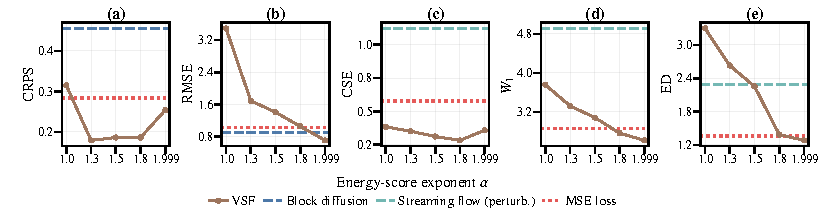
\includegraphics[width=\linewidth]{figures/ablation_plots/combined/crps_beta.pdf}
  \caption{Energy-score exponent. $\alpha$ ablation on (a)--(b)
  deterministic double pendulum and (c)--(e) stochastic R\"ossler. Dashed
  lines show the best overall baseline for each system; dotted lines show
  MSE-trained VSF. Three-seed means.}
  \label{fig:full-ablation-energy-score}
\end{figure}
\end{samepage}

\begin{samepage}
\paragraph{KL regularization.}
Figure~\ref{fig:full-ablation-kl} shows that performance is relatively robust
across the tested KL weights and remains better overall than SF, with an
intermediate weight giving the strongest aggregate result. The KL penalty must
balance retaining target-specific branch information in the training posterior
against aligning that posterior with the prior used for forecasting. When
regularization is too weak $(\beta_{\mathrm{KL}}=1e^{-3})$, the posterior--prior gap makes prior samples less
reliable at inference.

\begin{figure}[H]
  \centering
  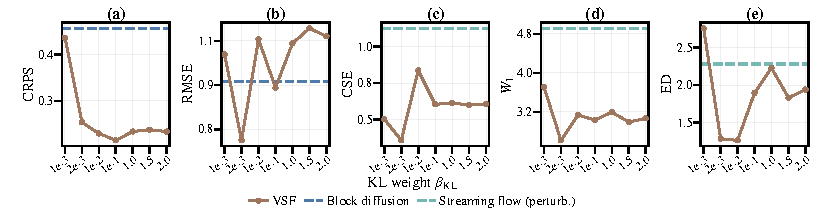
\includegraphics[width=\linewidth]{figures/ablation_plots/combined/kl_beta.pdf}
  \caption{KL regularization. $\beta_{\mathrm{KL}}$ ablation on
  (a)--(b) deterministic double pendulum and (c)--(e) stochastic R\"ossler.
  Dashed lines show the best overall baseline for each system. Three-seed means.}
  \label{fig:full-ablation-kl}
\end{figure}
\end{samepage}

\clearpage
\begin{samepage}
\paragraph{Latent contribution.}
Figure~\ref{fig:full-ablation-latent-weight} varies the latent contribution in
bottleneck-sum fusion. With no latent contribution, the model reduces to SF
and must rely on its evolving predicted history, so rollout errors can
accumulate. Every positive latent contribution improves overall performance
relative to SF by supplying a stable trajectory-level signal that is not
corrupted by previous prediction errors. An intermediate contribution performs
best, indicating that feedback through the recurrent bottleneck remains useful.
Although performance weakens at maximal latent contribution, the model still
retains state and physical-time conditioning and therefore remains robust;
maximal latent contribution does not make the predictor independent of the
physical state.

\begin{figure}[H]
  \centering
  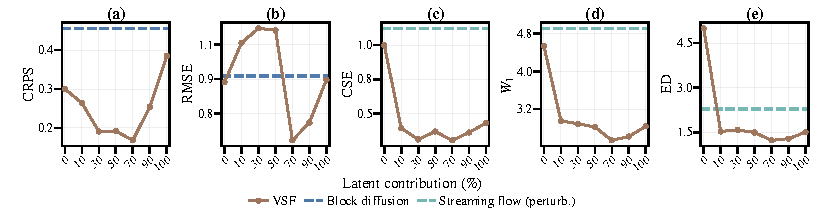
\includegraphics[width=\linewidth]{figures/ablation_plots/combined/latent_weight.pdf}
  \caption{Latent contribution. Bottleneck latent-weight ablation
  on (a)--(b) deterministic double pendulum and (c)--(e) stochastic R\"ossler.
  Dashed lines show the best overall baseline for each system. Three-seed means.}
  \label{fig:full-ablation-latent-weight}
\end{figure}
\end{samepage}

\begin{samepage}
\paragraph{Latent resampling.}
Figure~\ref{fig:full-ablation-resampling} compares sampling one latent for the
complete rollout with drawing a new latent at every forecast step. The two
strategies perform similarly early in the forecast, but the gap widens with
horizon in favor of a fixed latent. A rollout-wise fixed $\vz$ provides a
coherent trajectory-level source of uncertainty, whereas stepwise resampling
introduces temporally inconsistent perturbations and primarily harms
long-horizon probabilistic accuracy.

\begin{figure}[H]
  \centering
  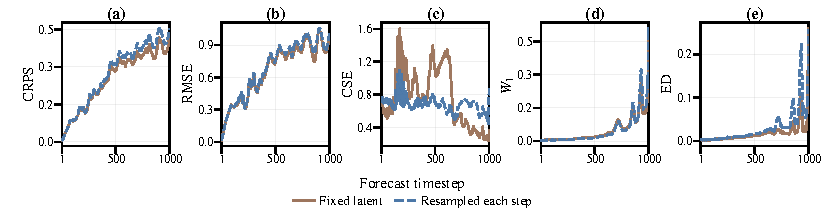
\includegraphics[width=\linewidth]{figures/ablation_plots/combined/latent_resampling.pdf}
  \caption{Latent resampling. Fixed rollout latent versus per-step
  resampling on (a)--(b) deterministic double pendulum and (c)--(e) stochastic
  R\"ossler. Three-seed means.}
  \label{fig:full-ablation-resampling}
\end{figure}
\end{samepage}

\clearpage


\paragraph{Latent-source and prior-alignment variants.}Figure~\ref{fig:latent-prior-alignment-ablation} separates three effects that
are otherwise coupled in VSF: stochastic latent conditioning,
future-conditioned variational training, and alignment of the training
posterior with the inference prior. Here
$p(\vz)=\mathcal N(\mathbf 0,\mathbf I_{d_z})$, and
$q_{\vphi}:=q_{\vphi}(\vz\mid\vu_s,\vx_s,s,\vh)$ is the
future-conditioned training posterior. Table~\ref{tab:latent-variant-definitions}
defines the four variants explicitly.

SF is the non-latent, MSE-trained reference. The three latent-conditioned
variants use the same decoder, $M$-sample generalized energy reconstruction
loss, and bottleneck latent contribution of $0.9$. Prior-latent SF is the
direct non-variational control: it uses prior samples during both training and
forecasting, with neither a posterior encoder nor a KL loss. In contrast,
Posterior VSF (no KL) remains variational because it uses the
future-conditioned posterior during training. Its prior samples at inference
are therefore unaligned with the training latents, creating a train--test
mismatch.

\begin{table}[t!]
  \centering
  \small
  \setlength{\tabcolsep}{18pt}
  \renewcommand{\arraystretch}{1.08}
  \caption{Definition of the latent-source and prior-alignment variants.}
  \begin{tabular}{@{}lcccc@{}}
    \toprule
    Variant & Training latent & \shortstack{Posterior\\encoder}
    & $\beta_{\mathrm{KL}}$ & Forecast latent \\
    \midrule
    SF & None & No & -- & None \\
    Prior-latent SF
    & $\vz^{(1:M)}\stackrel{\mathrm{iid}}{\sim}p(\vz)$
    & No & -- & $\vz\sim p(\vz)$, fixed \\
    Posterior VSF (no KL)
    & $\vz^{(1:M)}\stackrel{\mathrm{iid}}{\sim}q_{\vphi}$
    & Yes & $0$ & $\vz\sim p(\vz)$, fixed \\
    Full VSF
    & $\vz^{(1:M)}\stackrel{\mathrm{iid}}{\sim}q_{\vphi}$
    & Yes & $2\times10^{-3}$ & $\vz\sim p(\vz)$, fixed \\
    \bottomrule
  \end{tabular}

  \label{tab:latent-variant-definitions}
\end{table}

\begin{figure}[t!]
  \centering
  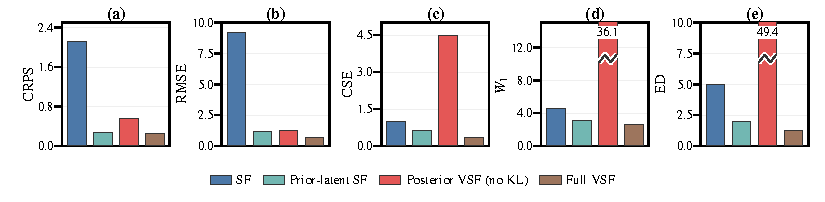
\includegraphics[width=\linewidth]{figures/ablation_plots/combined/latent_prior_alignment.pdf}
  \caption{Latent source and prior alignment. SF, Prior-latent SF,
  Posterior no-KL, and Full VSF on (a)--(b) deterministic double pendulum and
  (c)--(e) stochastic R\"ossler. Three-seed means; breaks mark labeled
  out-of-range values.}
  \label{fig:latent-prior-alignment-ablation}
\end{figure}



\paragraph{Does latent conditioning help?}
Prior-latent SF versus SF measures the benefit of the latent-conditioned,
multi-sample predictor without a learned posterior. Its improvement across
all  metrics shows that latent-conditioned prediction is already
useful without variational training.

\paragraph{Does variational training help?}
Full VSF has lower error than Prior-latent SF on all five metrics in Figure~\ref{fig:latent-prior-alignment-ablation}. Prior-latent SF samples training latents independently of the motion it must predict, making it harder to associate latent values with different possible futures. Full VSF instead infers latents from the observed local motion during training, helping different latent values represent different continuations. This is useful near a bifurcation, where nearly identical physical states can lead to different outcomes.


\paragraph{Why prior alignment matters.}
Full VSF versus Posterior no-KL isolates the role of the KL term when training
uses a future-conditioned posterior. Removing alignment degrades every metric,
especially the R\"ossler distributional scores. This is consistent with
train--test mismatch. Without KL
regularization, posterior codes may occupy regions or relative masses that are
not reproduced by the prior, so prior-sampled rollouts can miss or misweight
learned continuations. The gains from posterior-based training therefore
depend on aligning it with the forecasting prior.







\clearpage
\section{Rollout Error Plots}
\label{sec:rollout-error-plots}


\begin{figure}[h!]
  \centering
  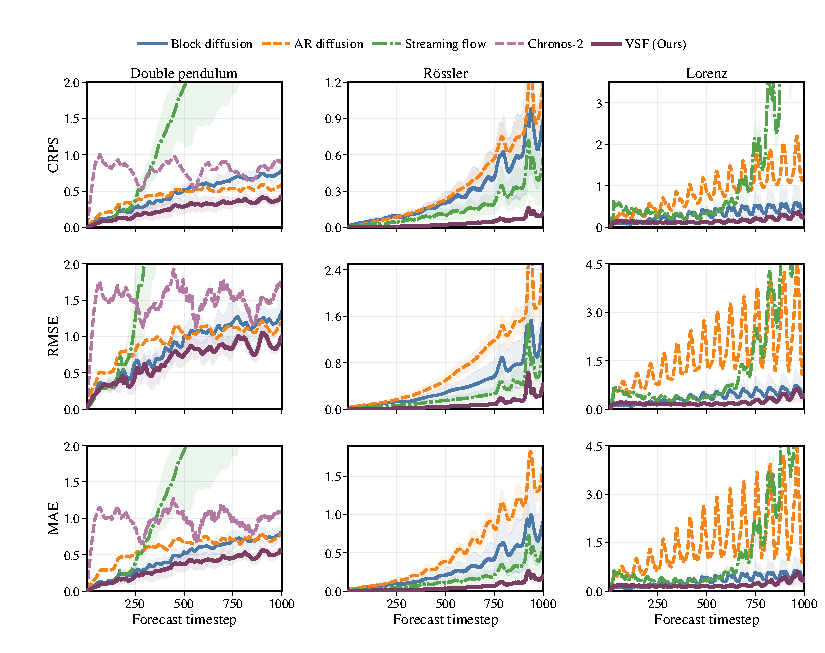
\includegraphics[width=\linewidth]{figures/rollout_error_plots/combined/rollout_errors_deterministic.pdf}
  \caption{Per-timestep error accumulation for 1,000-step deterministic
  forecasts. Columns show double pendulum, R\"ossler, and Lorenz; rows show
  CRPS, RMSE, and MAE. Curves and shaded bands report the mean and one standard
  deviation.}
  \label{fig:rollout-errors-deterministic}
\end{figure}
%  seed 100, 107, and 125

\begin{figure}[h!]
  \centering
  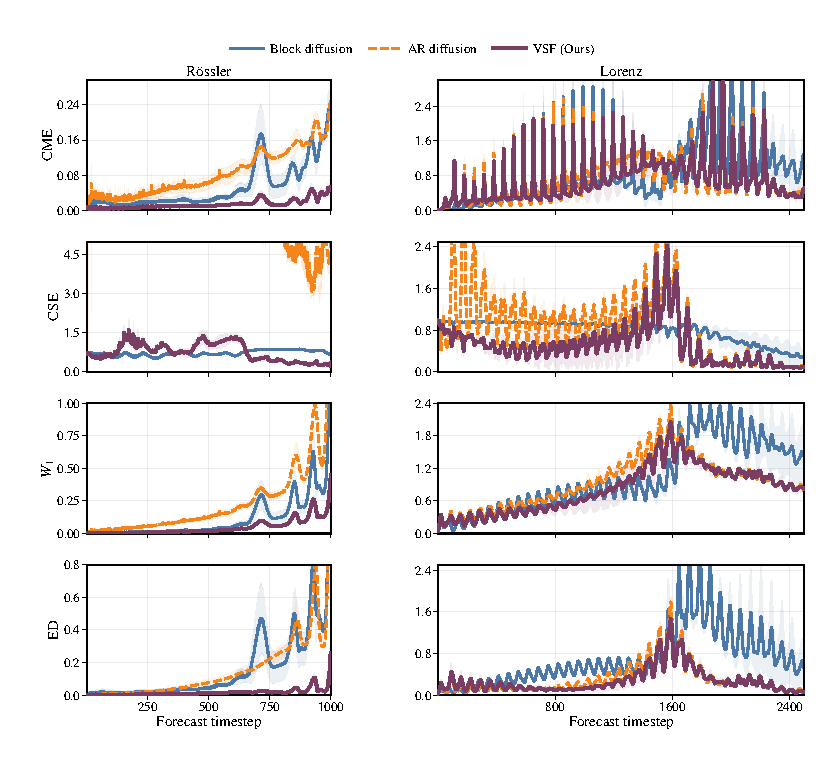
\includegraphics[width=\linewidth]{figures/rollout_error_plots/combined/rollout_errors_stochastic.pdf}
  \caption{Per-timestep distributional error for stochastic R\"ossler over
  1,000 steps and stochastic Lorenz over 2,500 steps. Columns show the two
  systems; rows show CME, CSE, marginal $W_1$, and marginal energy distance.
  Curves and shaded bands report the mean and one standard deviation. These per-timestep scores compare marginal
  standardized state distributions. They provide a different view from the joint whole-trajectory metrics in Tables~\ref{tab:forecasting_results}
  and~\ref{tab:stochastic-lorenz-2500}.}
  \label{fig:rollout-errors-stochastic}
\end{figure}




% Select one of the available instances by setting each flag to 01--05.
% Double pendulum uses two independent instances for its two regimes.
% These defaults may also be overridden before this file is input.
\providecommand{\DoublePendulumInstance}{01}
\providecommand{\DoublePendulumChaoticInstance}{02}
\providecommand{\DeterministicRosslerInstance}{01}
\providecommand{\DeterministicLorenzInstance}{01}
\providecommand{\StochasticRosslerInstance}{01}
\providecommand{\StochasticLorenzInstance}{01}

% Select five of the ten exported stochastic-Lorenz draws (01--10).
% Each selector is applied consistently to GT and every forecasting method.
\providecommand{\StochasticLorenzDrawOne}{01}
\providecommand{\StochasticLorenzDrawTwo}{08}
\providecommand{\StochasticLorenzDrawThree}{03}
\providecommand{\StochasticLorenzDrawFour}{04}
\providecommand{\StochasticLorenzDrawFive}{05}
\providecommand{\StochasticLorenzDrawSix}{06}
\providecommand{\StochasticLorenzDrawSeven}{07}



\newlength{\qualpanelwidth}
\newlength{\qualpanelheight}
\setlength{\qualpanelwidth}{0.225\linewidth}
\setlength{\qualpanelheight}{0.215\linewidth}
\newcommand{\qualplaceholder}{%
  \fbox{\parbox[c][\dimexpr\qualpanelheight-2\fboxsep-2\fboxrule\relax][c]{%
    \dimexpr\qualpanelwidth-2\fboxsep-2\fboxrule\relax}{%
    \centering\scriptsize Image\\placeholder}}%
}
\newcommand{\qualgraphic}[1]{%
  \includegraphics[
    width=\qualpanelwidth,
    height=\qualpanelheight,
    keepaspectratio
  ]{#1}%
}
\newcommand{\qualpanel}[1]{%
  \IfFileExists{#1.pdf}{%
    \qualgraphic{#1.pdf}%
  }{%
    \IfFileExists{#1.png}{\qualgraphic{#1.png}}{\qualplaceholder}%
  }%
}
\newcommand{\quallabelfont}{\normalfont\small}
\newcommand{\qualheader}[1]{{\quallabelfont\shortstack{#1}}}
\newcommand{\qualrowlabel}[1]{%
  \parbox[b][\qualpanelheight][c]{2em}{%
    \centering
    \rotatebox[origin=c]{90}{{\quallabelfont\shortstack{#1}}}%
  }%
}
\newcommand{\qualdeterministicrow}[2]{%
  \qualrowlabel{#1}
  & \qualpanel{#2_samples_gt}
  & \qualpanel{#2_samples_vsf}
  & \qualpanel{#2_mean_vsf}
  & \qualpanel{#2_samples_streaming_flow}
  & \qualpanel{#2_samples_block_diffusion} \\[0.2em]
}
\newcommand{\qualzoomrow}[2]{%
  \qualrowlabel{#1}
  & \multicolumn{5}{c}{%
    \parbox[b][\qualpanelheight][c]{%
      \dimexpr5\qualpanelwidth+8\tabcolsep\relax}{%
      \centering
      \includegraphics[
        width=\linewidth,
        height=\qualpanelheight,
        keepaspectratio
      ]{#2}%
    }%
  } \\[0.2em]
}

\newcommand{\stochasticlorenzrow}[2]{%
  {\quallabelfont #1}
  & \qualpanel{figures/lorenz_stochastic/instance_\StochasticLorenzInstance%
      _stochastic_lorenz_draw_#2_gt}
  & \qualpanel{figures/lorenz_stochastic/instance_\StochasticLorenzInstance%
      _stochastic_lorenz_draw_#2_vsf}
  & \qualpanel{figures/lorenz_stochastic/instance_\StochasticLorenzInstance%
      _stochastic_lorenz_draw_#2_streaming_flow}
  & \qualpanel{figures/lorenz_stochastic/instance_\StochasticLorenzInstance%
      _stochastic_lorenz_draw_#2_block_diffusion}
  & \qualpanel{figures/lorenz_stochastic/instance_\StochasticLorenzInstance%
      _stochastic_lorenz_draw_#2_ar_diffusion} \\[0.15em]
}


\clearpage
\section{Trajectory Forecast Visualizations}
\label{sec:qualitative-trajectory-forecasts}
We compare sampled forecast trajectories across the evaluated systems and
baselines. For the deterministic systems, we additionally show the VSF
ensemble predictive mean.

\begin{figure}[h!]
  \centering
  \begingroup
  \setlength{\qualpanelwidth}{0.18\linewidth}
  \setlength{\qualpanelheight}{0.18\linewidth}
  \setlength{\tabcolsep}{0.75pt}
  \renewcommand{\arraystretch}{1.0}
  \begin{tabular}{@{}c*{5}{c}@{}}
    & \qualheader{GT}
    & \qualheader{VSF (Ours)}
    & \qualheader{VSF ensemble}
    & \qualheader{SF}
    & \qualheader{Block diffusion} \\[0.15em]
    \qualdeterministicrow{Double \\pendulum}{figures/double_pendulum/instance_%
      \DoublePendulumInstance_deterministic_double_pendulum}
    \qualzoomrow{Double\\pendulum}{figures/zoom_double_pendulum.pdf}
    \qualzoomrow{R\"ossler}{figures/zoom_deterministic_rossler.pdf}
    \qualzoomrow{Lorenz}{figures/zoom_deterministic_lorenz.pdf}
  \end{tabular}
  \endgroup
  \caption{Qualitative forecasts on the deterministic systems. Columns show
  ground truth (GT), VSF samples, the VSF ensemble predictive mean, SF, and
  block diffusion. Sample panels contain $N=10$ trajectories; the VSF ensemble is the mean of the samples. The last three rows magnify highlighted regions of the chaotic double-pendulum, R\"ossler, and Lorenz forecasts.}
  \label{fig:qualitative-deterministic}
  \label{fig:main-chaotic-double-pendulum}
  \label{fig:qualitative-deterministic-double-pendulum-chaotic}
  \label{fig:qualitative-deterministic-rossler}
  \label{fig:qualitative-deterministic-lorenz}
\end{figure}

\begin{figure}[h!]
  \centering
  \begingroup
  \setlength{\qualpanelwidth}{0.18\linewidth}
  \setlength{\qualpanelheight}{0.17\linewidth}
  \setlength{\tabcolsep}{1pt}
  \renewcommand{\arraystretch}{1.05}
  \begin{tabular}{@{}c*{5}{c}@{}}
    \qualheader{Sample}
    & \qualheader{GT}
    & \qualheader{VSF (Ours)}
    & \qualheader{SF}
    & \qualheader{Block\\diffusion}
    & \qualheader{AR\\diffusion} \\
    \stochasticlorenzrow{1}{\StochasticLorenzDrawOne}
    \stochasticlorenzrow{2}{\StochasticLorenzDrawTwo}
    \stochasticlorenzrow{3}{\StochasticLorenzDrawThree}
    \stochasticlorenzrow{4}{\StochasticLorenzDrawFour}
    \stochasticlorenzrow{5}{\StochasticLorenzDrawSeven}
  \end{tabular}
  \endgroup
  \caption{Visualization samples from the ground truth and generated trajectories for the partially observed stochastic Lorenz.}
  \label{fig:qualitative-stochastic-lorenz}
\end{figure}



% \clearpage
% \section{World-Model Latent-Trajectory Visualizations}
% \label{sec:world-model-latent-trajectory-visualizations}

% \begin{figure}[H]
%   \centering
%   \begin{tikzpicture}
%     \node[inner sep=0pt,outer sep=0pt] (arp-panel) {%
%       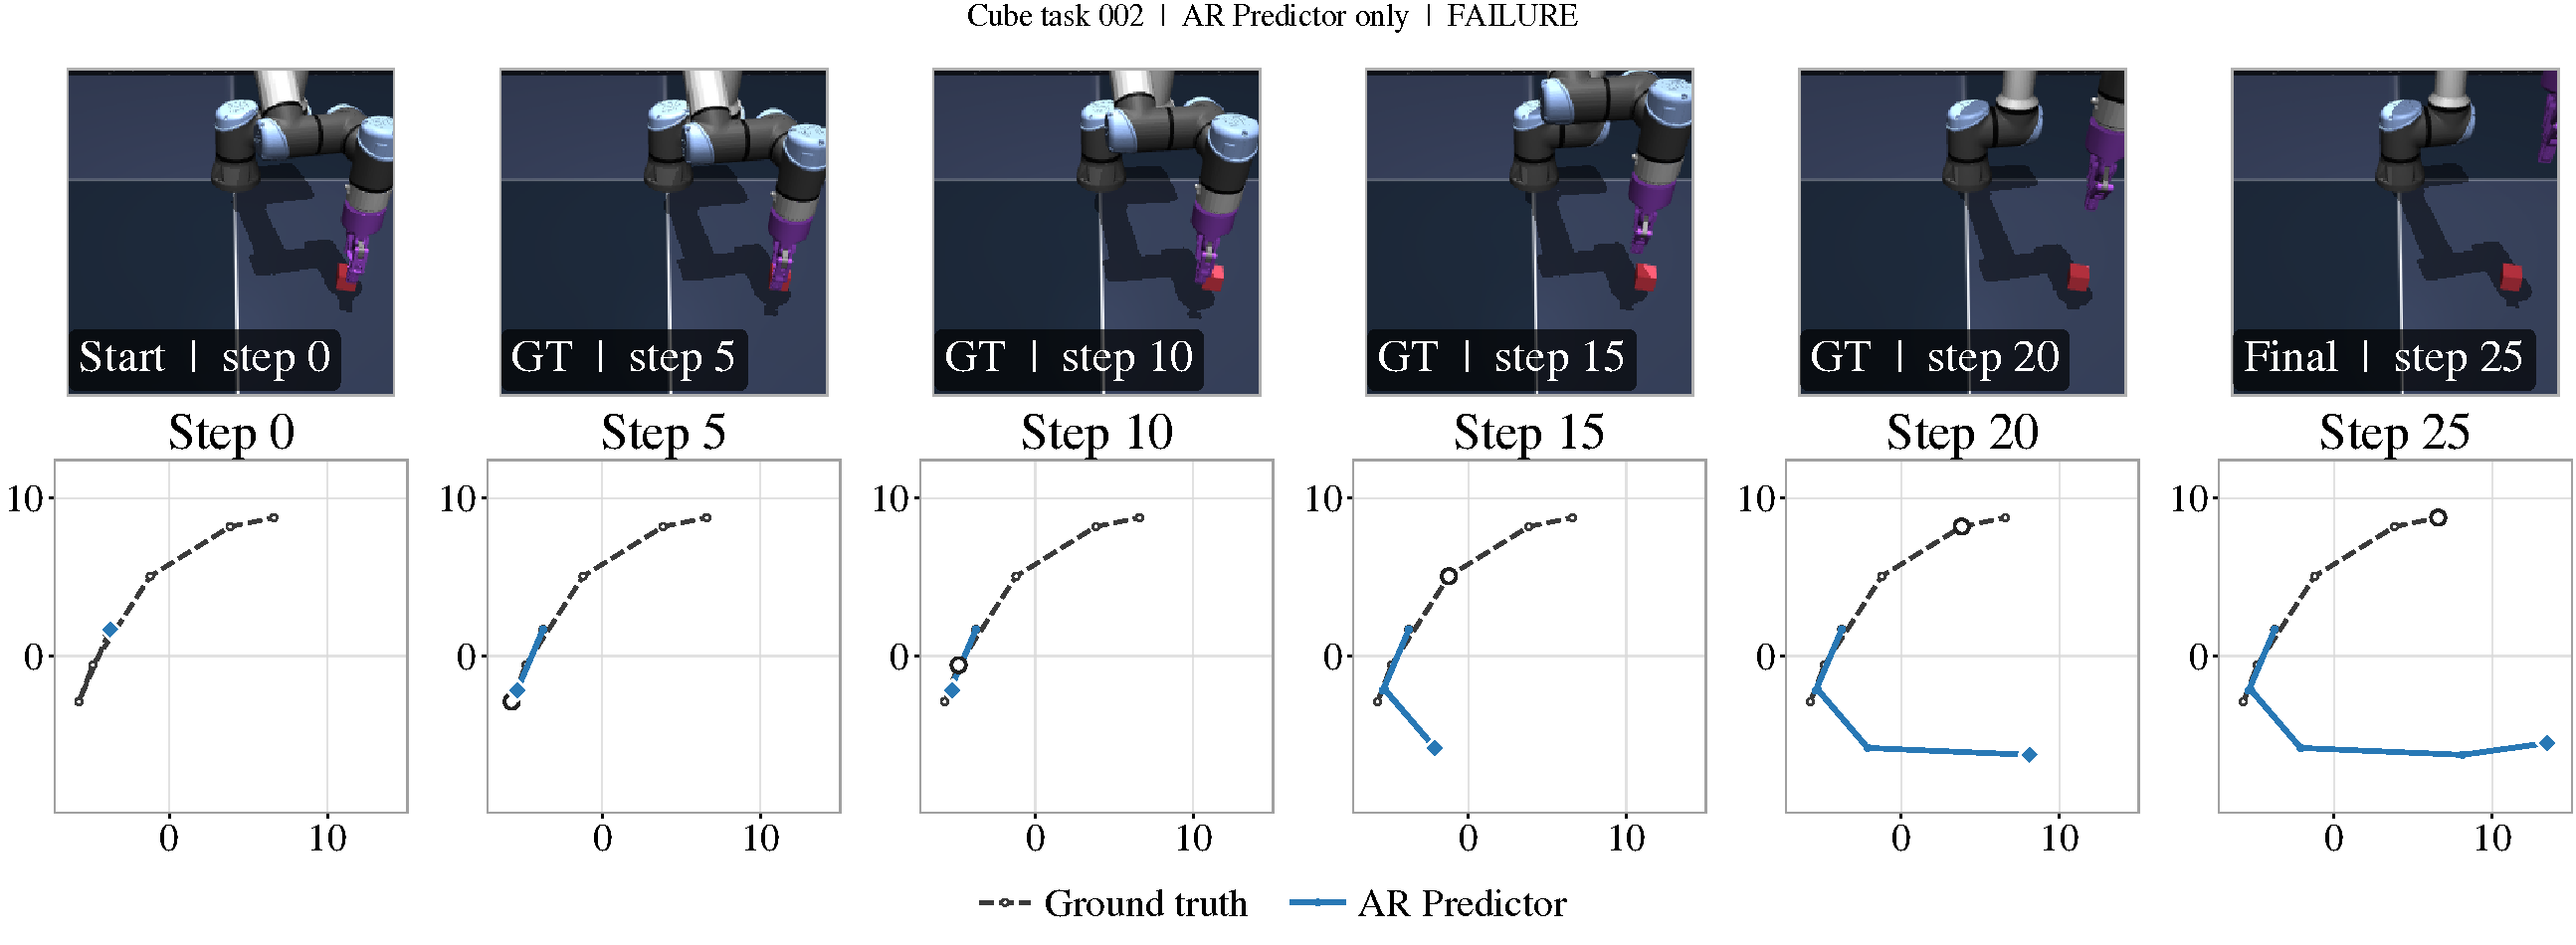
\includegraphics[
%         width=0.78\linewidth,
%         trim={0bp 0bp 0bp 20bp},
%         clip
%       ]{figures/wm/cube_task_002_arp_latent_trajectory.pdf}%
%     };
%     \node[
%       anchor=south west,
%       inner sep=0pt,
%       outer sep=0pt,
%       xshift=0pt,
%       yshift=2pt,
%       font=\normalfont\normalsize
%     ] at (arp-panel.north west) {(a)};
%   \end{tikzpicture}\par\nointerlineskip
%   \begin{tikzpicture}
%     \node[inner sep=0pt,outer sep=0pt] (vsf-panel) {%
%       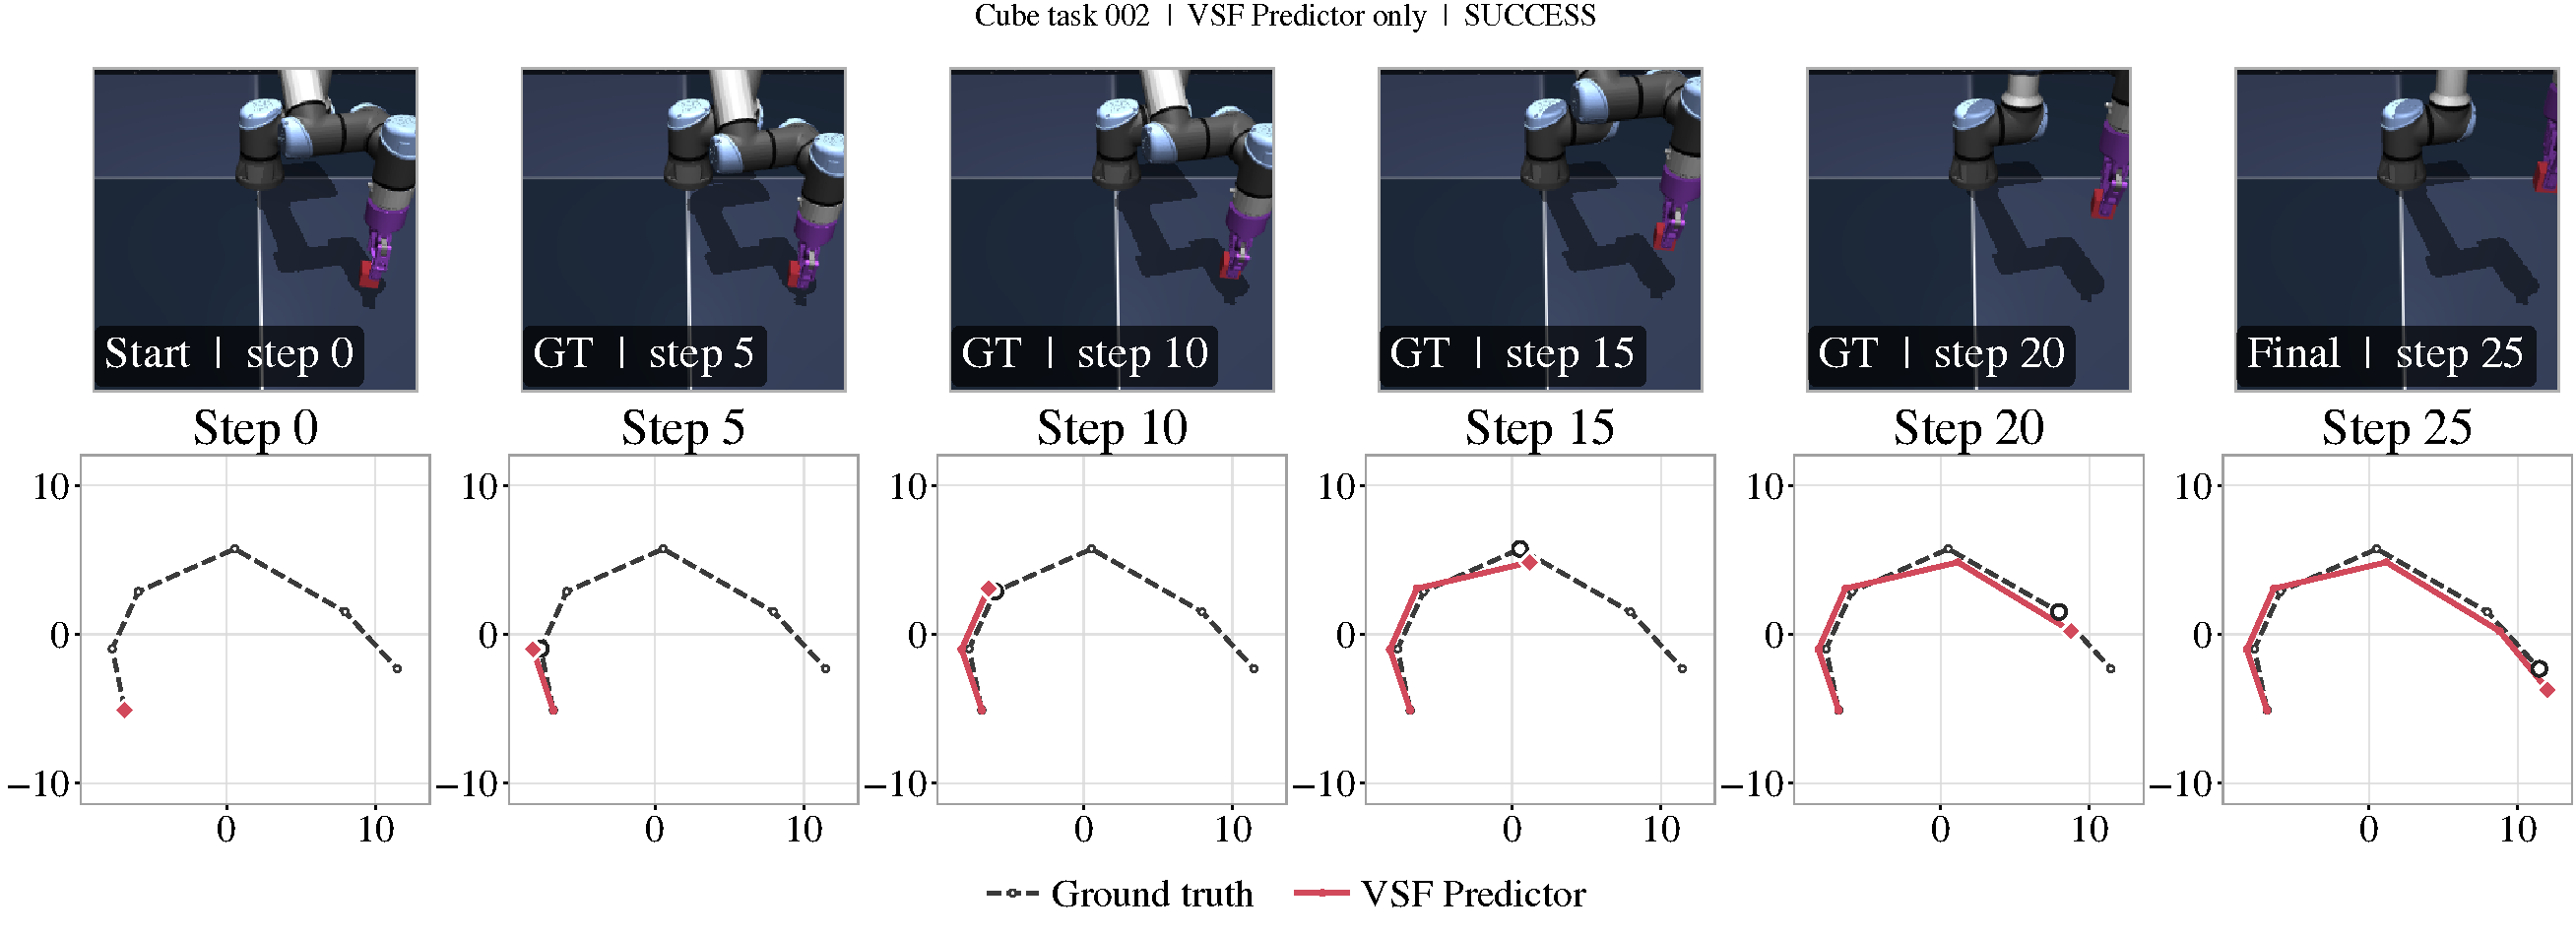
\includegraphics[
%         width=0.78\linewidth,
%         trim={0bp 0bp 0bp 20bp},
%         clip
%       ]{figures/wm/cube_task_002_vsf_latent_trajectory.pdf}%
%     };
%     \node[
%       anchor=south west,
%       inner sep=0pt,
%       outer sep=0pt,
%       xshift=0pt,
%       yshift=2pt,
%       font=\normalfont\normalsize
%     ] at (vsf-panel.north west) {(b)};
%   \end{tikzpicture}
%   \caption{The top row shows the ground-truth observations during rollout. The bottom row compares the predicted and ground-truth latent trajectories after joint-PCA projections. (a) The AR Predictor trajectory diverges
%   and the rollout fails. (b) The VSF Predictor trajectory follows the
%   ground-truth trajectory and the rollout succeeds.}
%   \label{fig:wm-cube-task-002-latent-trajectories}
% \end{figure}

% \begin{figure}[H]
%   \centering
%   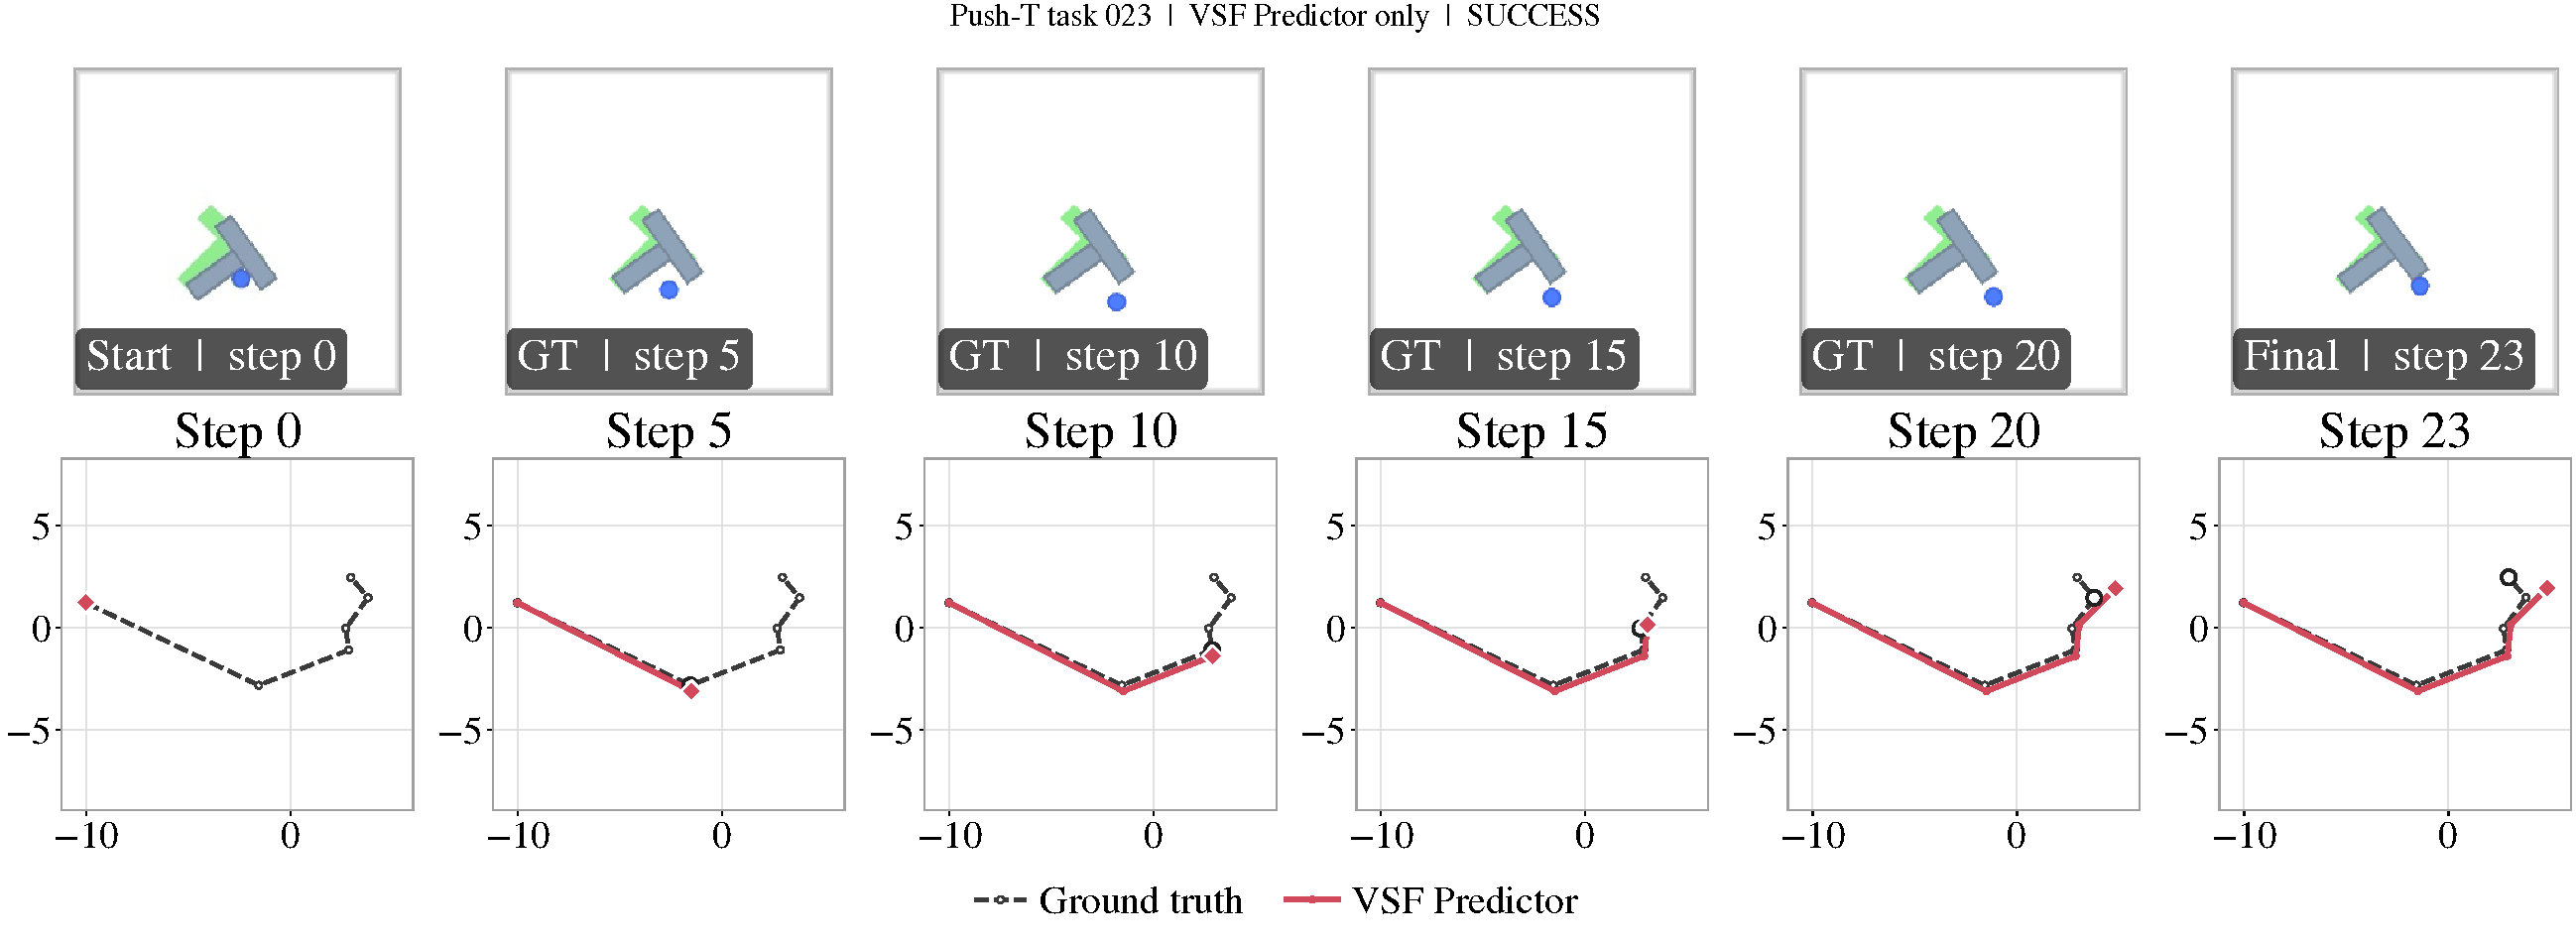
\includegraphics[
%     width=0.78\linewidth,
%     trim={0bp 0bp 0bp 20bp},
%     clip
%   ]{figures/wm/pusht_task_023_vsf_latent_trajectory.pdf}
%   \caption{Qualitative PushT result. VSF action-conditioned predicted latent
%   trajectory follows the ground-truth trajectory in a successful rollout.}
%   \label{fig:wm-vsf-pusht-qualitative}
% \end{figure}

% \begin{figure}[H]
%   \centering
%   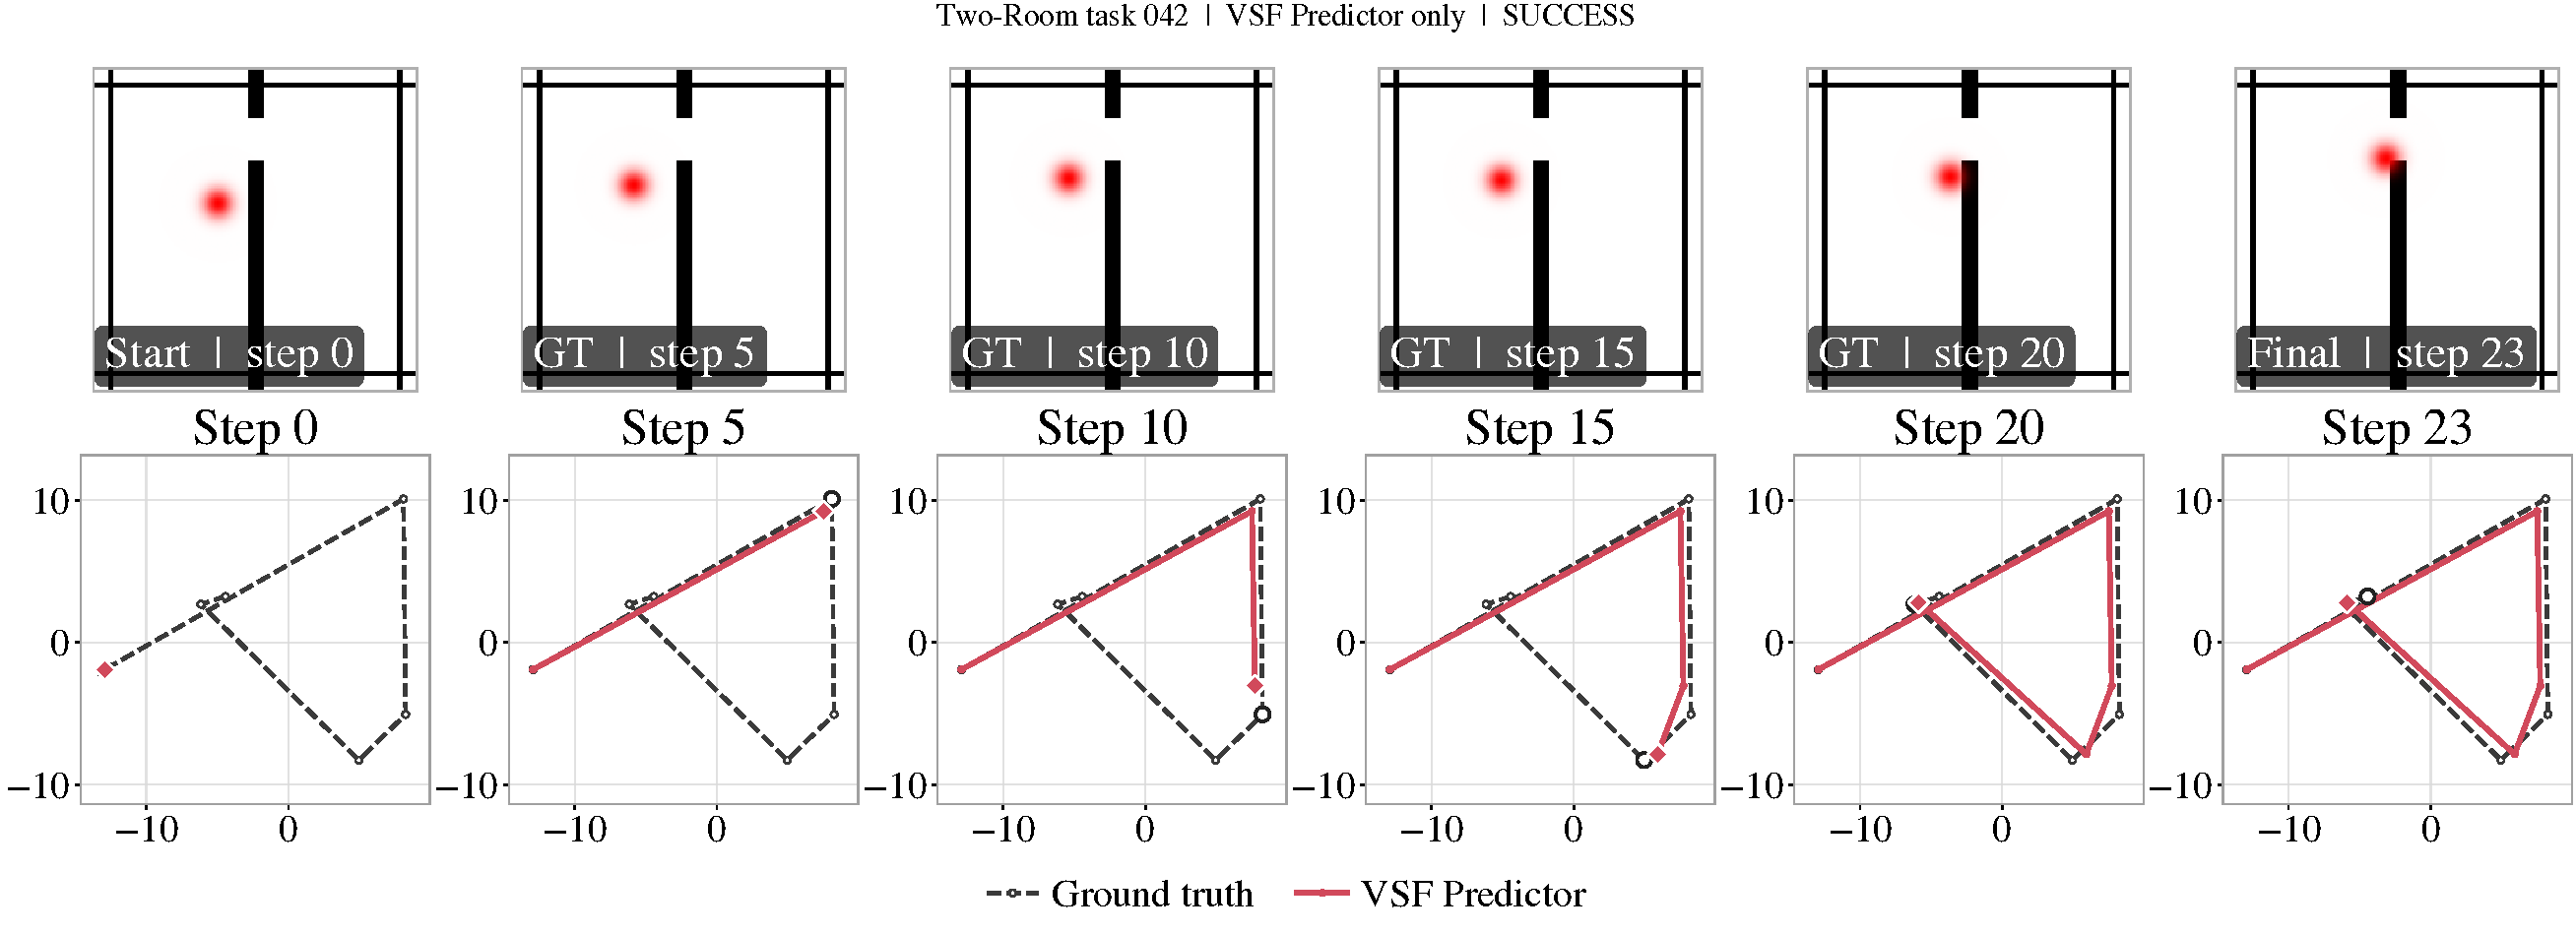
\includegraphics[
%     width=0.78\linewidth,
%     trim={0bp 0bp 0bp 20bp},
%     clip
%   ]{figures/wm/tworoom_task_042_vsf_latent_trajectory.pdf}
%   \caption{Qualitative TwoRoom result. VSF action-conditioned predicted latent
%   trajectory follows the ground-truth trajectory in a successful rollout.}
%   \label{fig:wm-vsf-reacher-qualitative}
% \end{figure}

\clearpage
\section{World-Model Latent-Trajectory Visualizations}
\label{sec:world-model-latent-trajectory-visualizations}

\begin{figure}[H]
  \centering
  \begin{tikzpicture}
    \node[inner sep=0pt,outer sep=0pt] (arp-panel) {%
      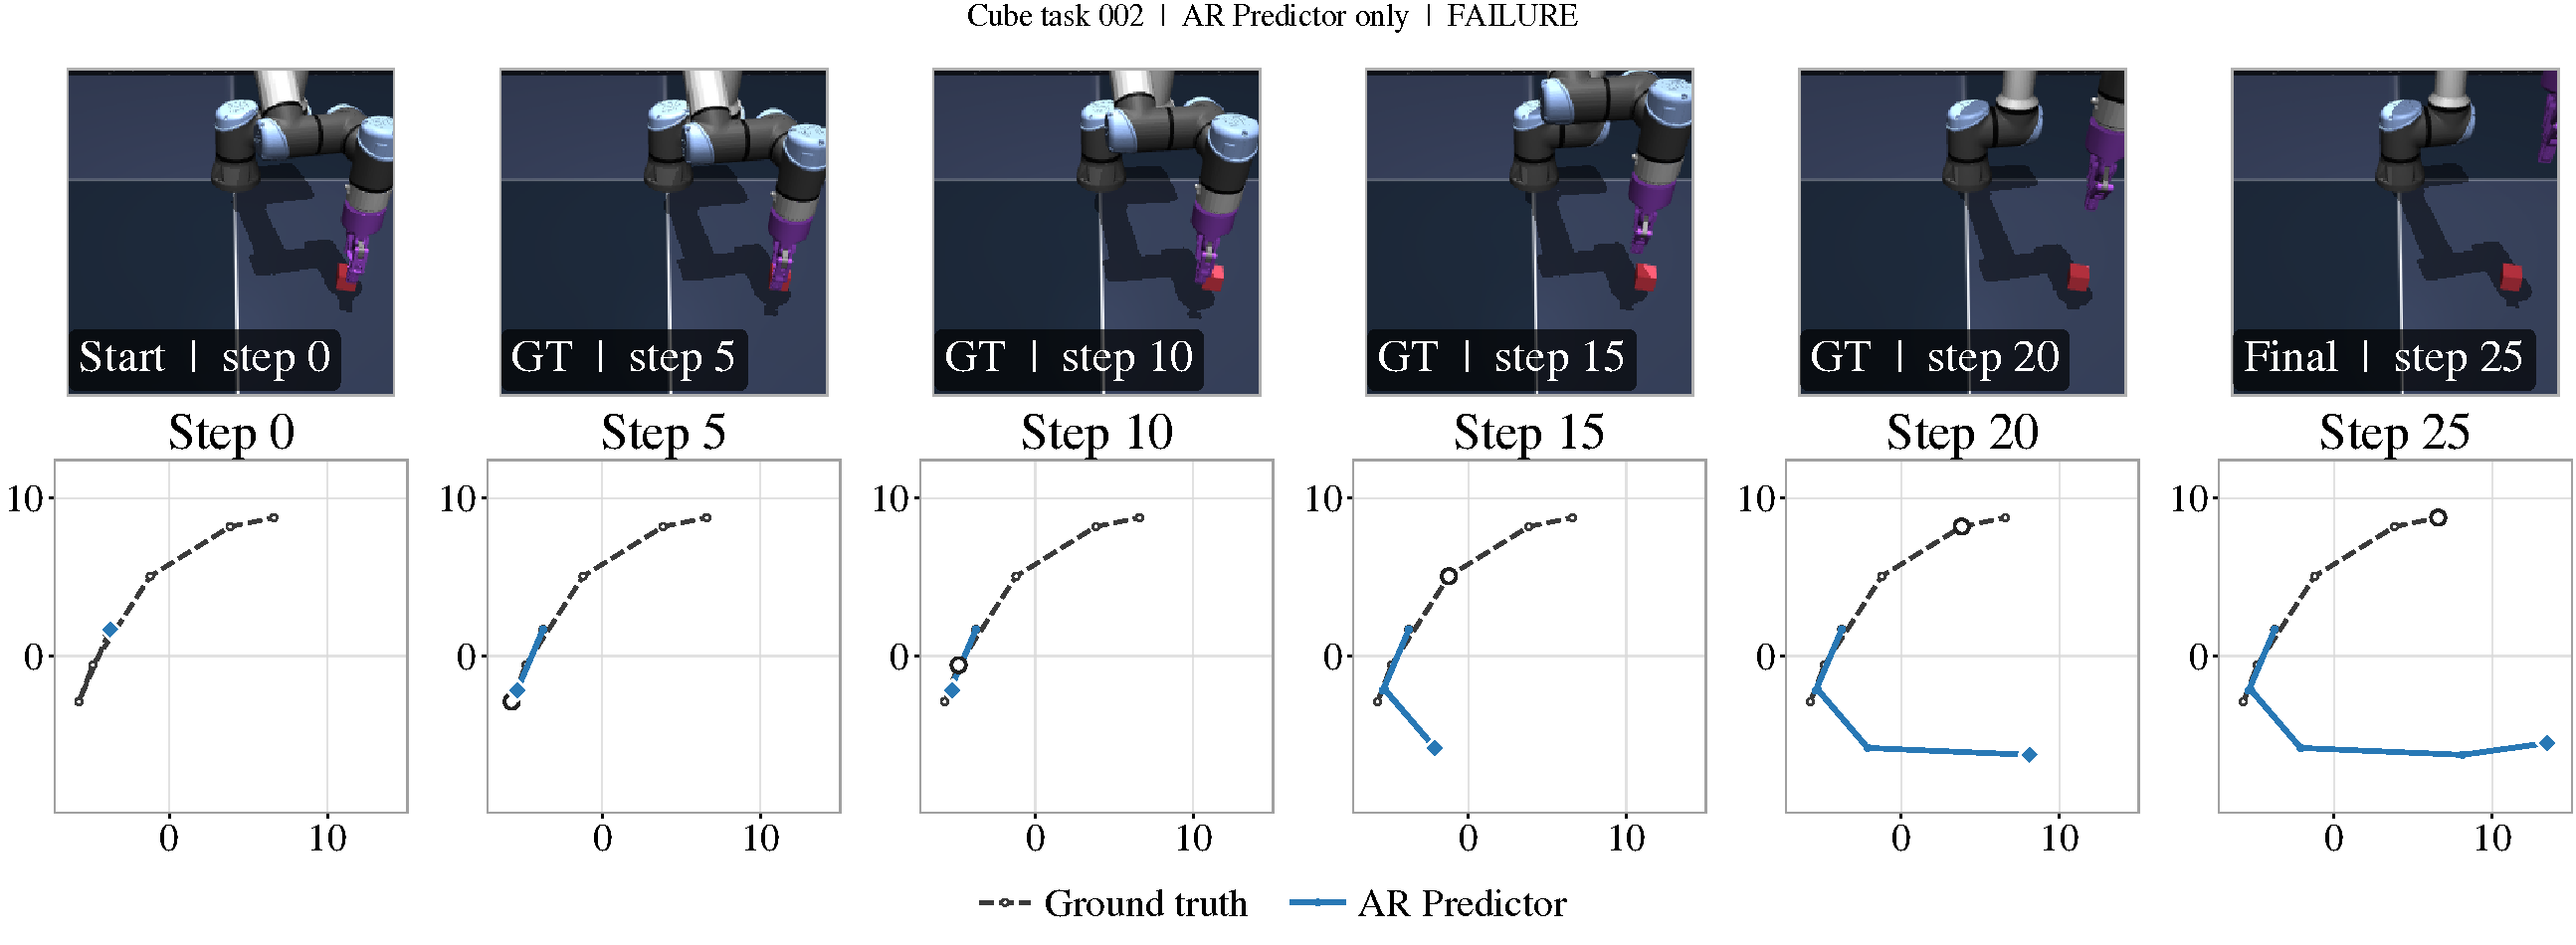
\includegraphics[
        width=\linewidth,
        trim={0bp 0bp 0bp 20bp},
        clip
      ]{figures/wm/cube_task_002_arp_latent_trajectory.pdf}%
    };
    \node[
      anchor=south west,
      inner sep=0pt,
      outer sep=0pt,
      xshift=0pt,
      yshift=2pt,
      font=\normalfont\normalsize
    ] at (arp-panel.north west) {(a)};
  \end{tikzpicture}\par\nointerlineskip
  \begin{tikzpicture}
    \node[inner sep=0pt,outer sep=0pt] (vsf-panel) {%
      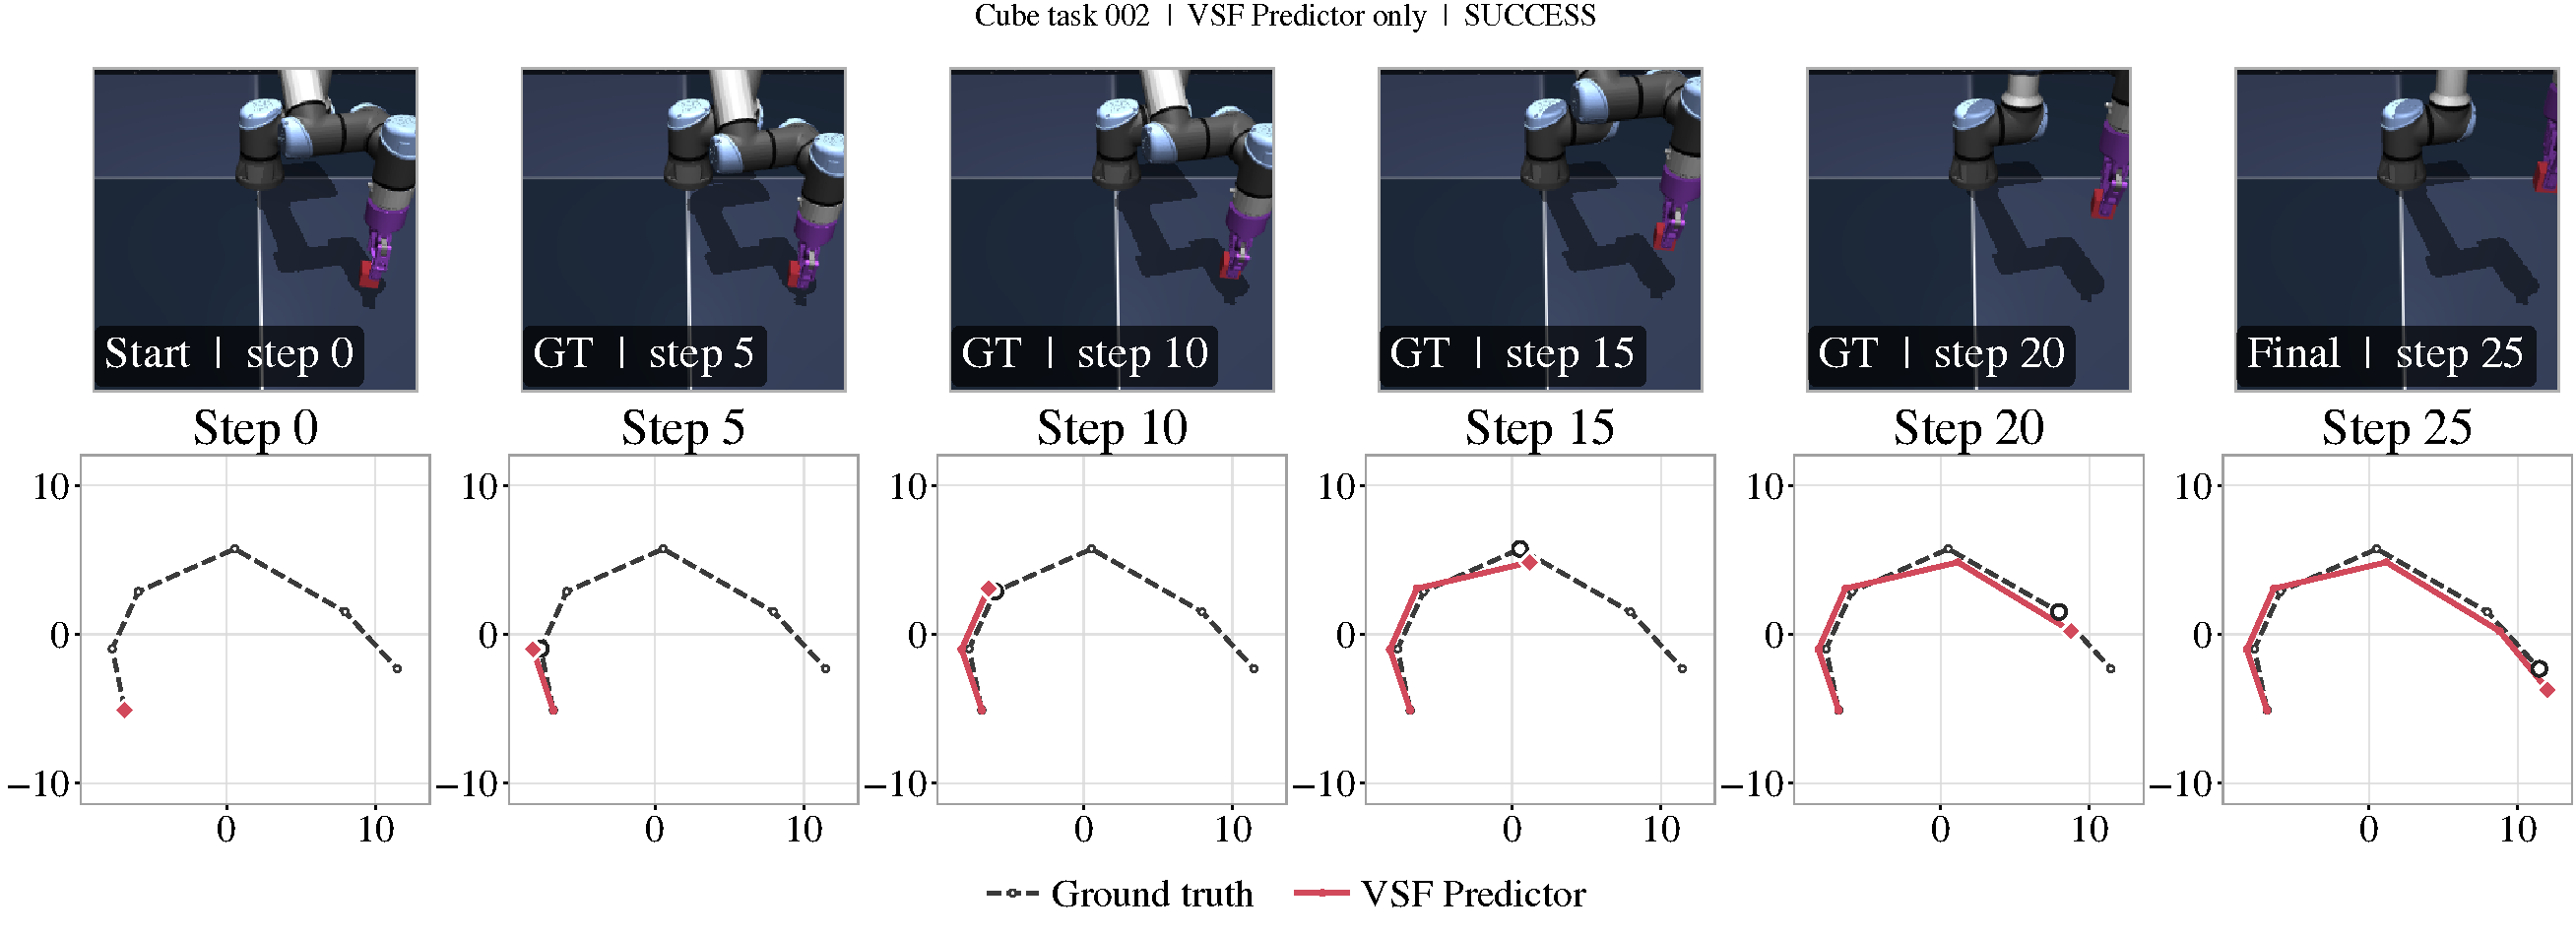
\includegraphics[
        width=\linewidth,
        trim={0bp 0bp 0bp 20bp},
        clip
      ]{figures/wm/cube_task_002_vsf_latent_trajectory.pdf}%
    };
    \node[
      anchor=south west,
      inner sep=0pt,
      outer sep=0pt,
      xshift=0pt,
      yshift=2pt,
      font=\normalfont\normalsize
    ] at (vsf-panel.north west) {(b)};
  \end{tikzpicture}
  \caption{The top row shows the ground-truth observations during rollout. The bottom row compares the predicted and ground-truth latent trajectories after joint-PCA projections. (a) The AR Predictor trajectory diverges
  and the rollout fails. (b) The VSF Predictor trajectory follows the
  ground-truth trajectory and the rollout succeeds.}
  \label{fig:wm-cube-task-002-latent-trajectories}
\end{figure}

\clearpage
\begin{figure}[H]
  \centering
  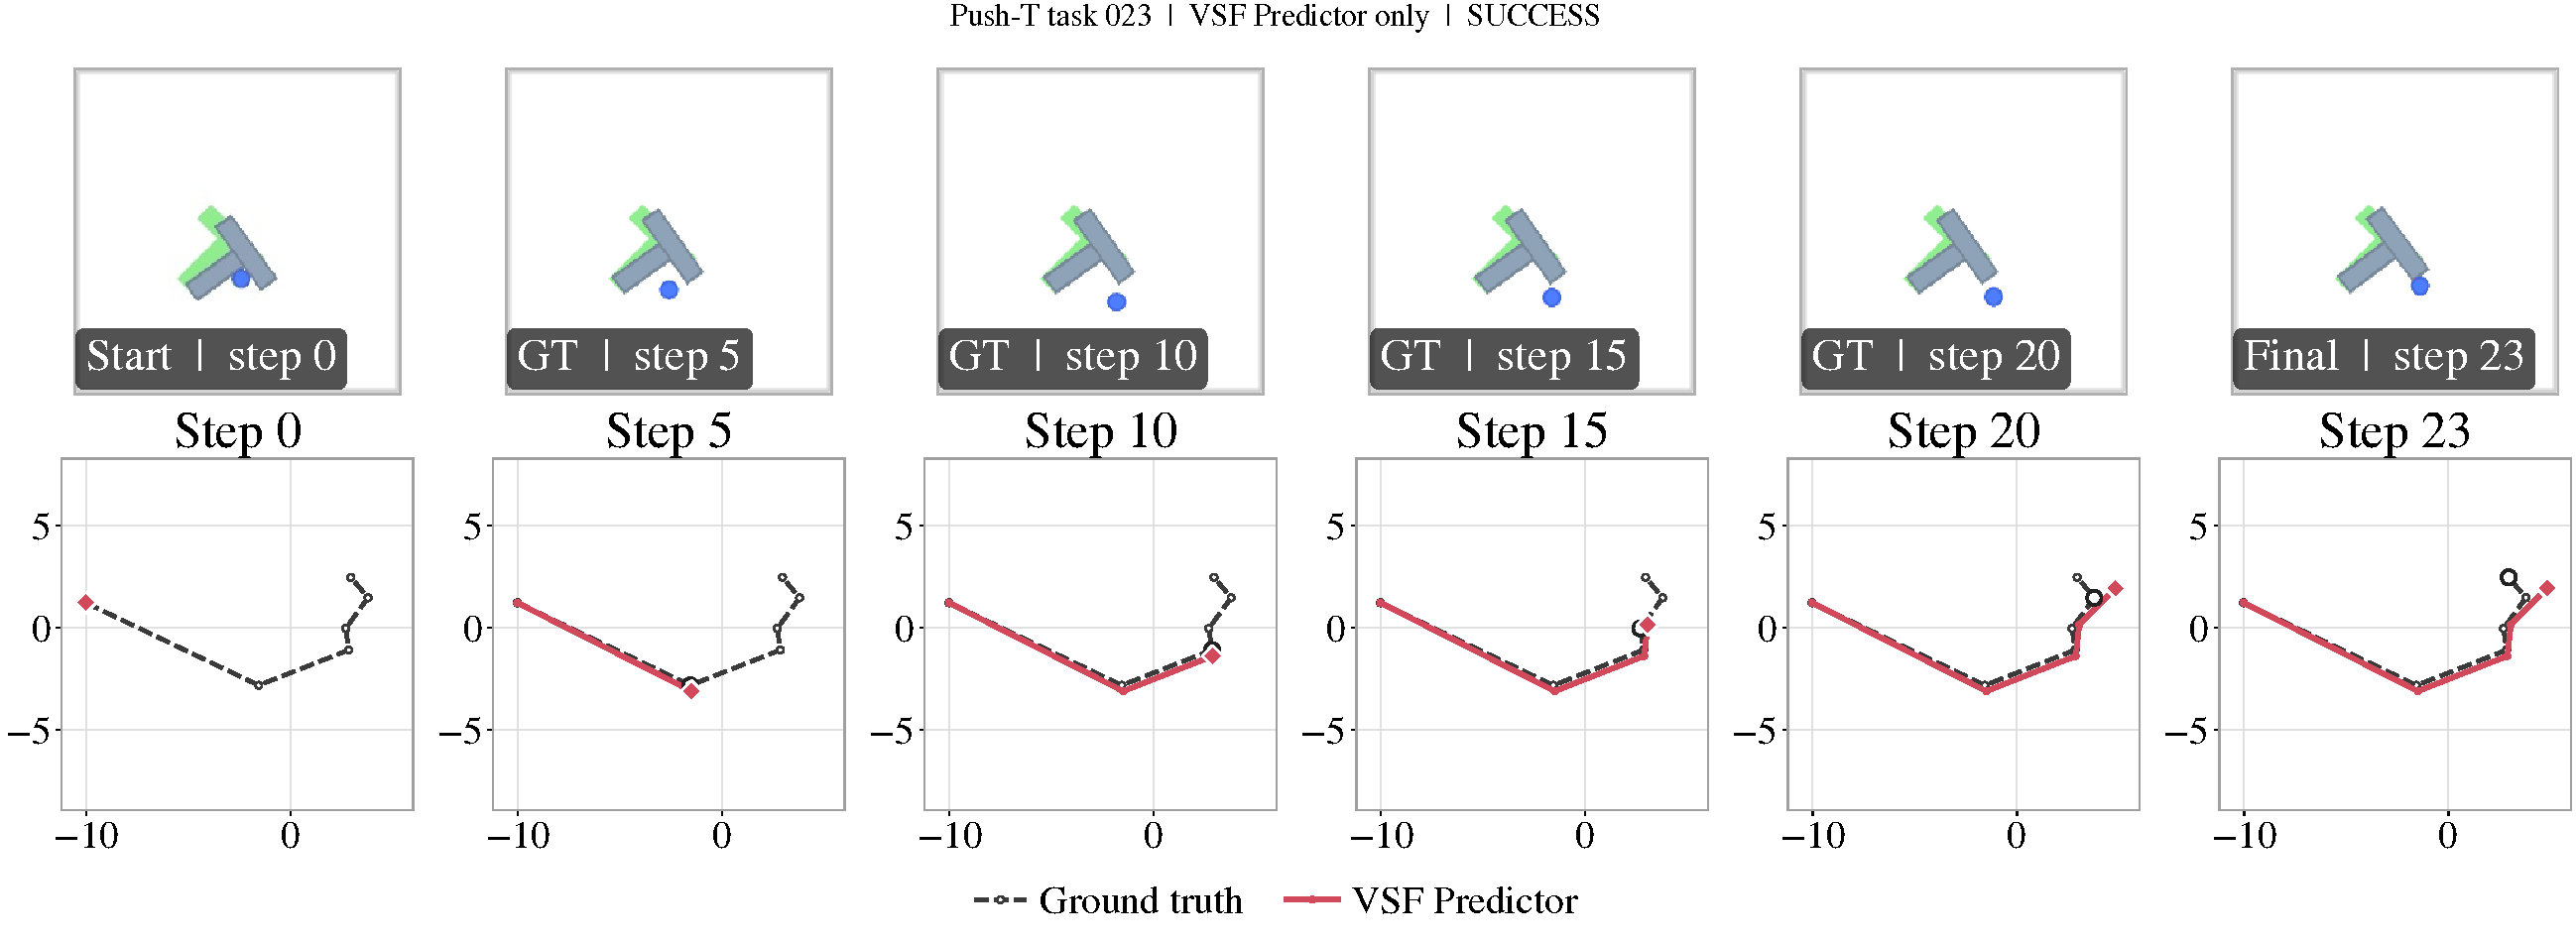
\includegraphics[
    width=\linewidth,
    trim={0bp 0bp 0bp 20bp},
    clip
  ]{figures/wm/pusht_task_023_vsf_latent_trajectory.pdf}
  \caption{Qualitative PushT result. VSF action-conditioned predicted latent
  trajectory follows the ground-truth trajectory in a successful rollout.}
  \label{fig:wm-vsf-pusht-qualitative}
\end{figure}

\begin{figure}[H]
  \centering
  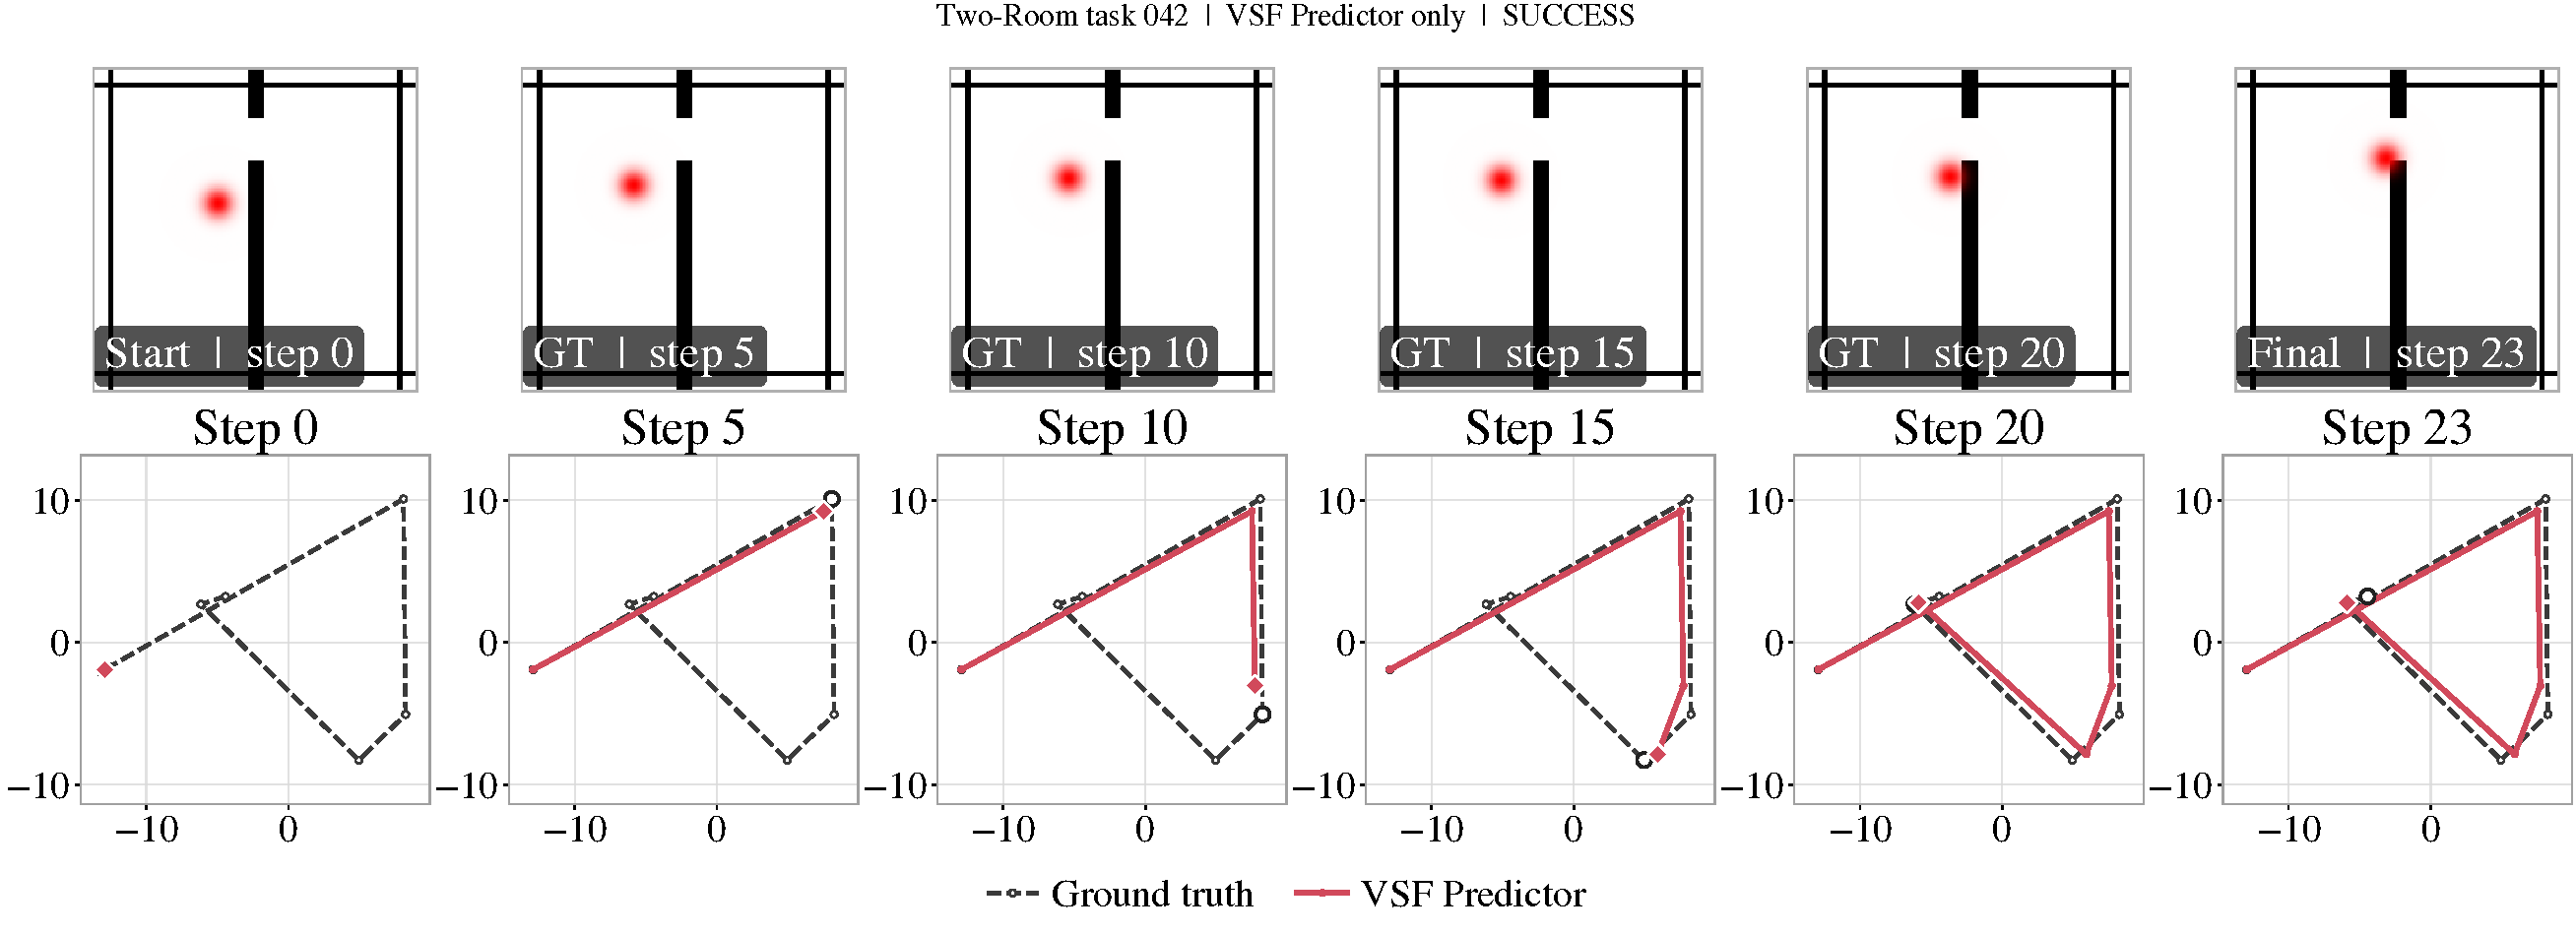
\includegraphics[
    width=\linewidth,
    trim={0bp 0bp 0bp 20bp},
    clip
  ]{figures/wm/tworoom_task_042_vsf_latent_trajectory.pdf}
  \caption{Qualitative TwoRoom result. VSF action-conditioned predicted latent
  trajectory follows the ground-truth trajectory in a successful rollout.}
  \label{fig:wm-vsf-reacher-qualitative}
\end{figure}
